\chapter{Introduction}
The thesis is organized as follows. The theoretical background, from the concept of the gauge invariance, the electroweak theory to the Higgs mechanism, will be introduced. The experimental perspective and an overview of the searched decays $\cPZ / \PH\to\JPsi\ \gamma$ are followed. Chapter~\ref{Chap:CMS} will briefly mention the experiment apparatus, with the object reconstruction. In Chapter~\ref{Chap:Ana}, the analysis procedure and methods, including data and simulated samples, the object identification, background and signal models construction, systematic uncertainties estimation, and the statistical methods, are described in detail. Chapter~\ref{Chap:Results} represents the results of this analysis, as well as the possible improvements.
  
\section{The standard model of particle physics}
The standard model (SM) of particle physics provides so far the most effective and appropriate theory framework to describe the fundamental constituents of the Universe, and the interactions between them, the force\footnotemark, which are carried by the gauge boson. The last piece of the SM is the Higgs boson, which is the manifestation of the mechanism by which particles acquire masses. 
\footnotetext{The interactions here do not include the gravitational force. In the following text, ''the interactions in the SM`` will simply refer to the electromagnetic, weak, and strong forces. }

There are twelve fundamental fermions in the SM, and are categorized into quarks and leptons by the types of interactions they experience. All the fermions involve in the weak interaction, which is mediated by the $\Wpm$ and $\cPZ$ bosons. Except for the electrically neutral neutrinos, the remaining nine fermions participate in the electromagnetic interaction, which is mediated by the photon $\gamma$. The theory of the electromagnetic interaction is the Quantum Electrodynamics (QED), which is the most accurately tested physics theory. 
The above two interactions can be unified into the Electro-Weak theory (EW), and will be described later in the text.  
Only the quarks carry the color charge and undergo the strong interaction, which is mediated by the gluons $\cPg$. The theory for the strong interaction is the Quantum Chromodynamics (QCD). The color is a label for the three orthogonal states in the SU(3) symmetry group of the QCD.
Quarks are always bound together to form hadrons, which can either be mesons (consist of a quark and a anti-quark) or baryons (consist of three quarks). This is the nature of the QCD, called color confinement -- quarks are always observed to be confined to bound colorless states. An overview of QCD can be found in the lecture~\cite{Skands:2012ts} and will not be discussed in this thesis. The elementary particles, and their basic properties, are summarized in Fig.~\ref{fig:SMgraph}.

\begin{figure}[!ht]
  \begin{center}  
    \includegraphics[width=1.0\textwidth]{Fig/model-physics}\\
    \caption{The elementary particles of SM, with the three generations of fermions, four gauge bosons, and the Higgs boson. \label{fig:SMgraph}} 
  \end{center}
\end{figure} 

\subsection{Gauge invariance}
In the context of Quantum Field Theory (QFT), particles are described by excitations of a quantum field which satisfies the quantum field equation. In a continuous system, the \emph{field} represents the generalized coordinates at each point in space-time, and therefore is written in the form of a continuous function. The dynamics of the field is often expressed by the Lagrangian density $\mathcal{L}(\phi_{i},\partial_{\mu}\phi_{i})$ where $\phi_{i}$ is the field. Later in the text a simplified term ''the Lagrangian`` will be used to replace the Lagrangian density.
The equation of motion describing the dynamics of the field can be derived from the Euler-Lagrange equation 
\begin{equation}
\partial_{\mu}\bigg(\frac{\partial\mathcal{L}}{\partial(\partial_{\mu}\phi_{i})}\bigg)-\frac{\partial\mathcal{L}}{\partial\phi_{i}}=0.
\end{equation}

The three interactions, QED, weak, and QCD, can be derived by requiring the \emph{local guage invariance}: the Lagrangian is invariant under the \emph{local phase transformation} of the fields,
\begin{equation}
\psi(x) \ \to\ \psi^{\prime}(x) = \hat{U(x)}\psi(x) = \mathrm{e}^{iq\chi(x)}\psi(x).
\end{equation}
The Lagrangian for a free spin-$\frac{1}{2}$ particle (referred to as free Lagrangian)
\begin{equation}
\label{eqn:LagSpinhalf}
\mathcal{L}_{\text{free}}=i\bar{\psi}\gamma^{\mu}\partial_{\mu}\psi-m\bar{\psi}\psi.
\end{equation}
With the U(1) local gauge transformation, Eq.~\ref{eqn:LagSpinhalf} becomes
\begin{equation}
\label{eqn:LagSpinhalf_LocalTrans}
\mathcal{L}_{\text{free}}\ \to\ \mathcal{L}_{\text{free}}^{\prime} = \mathcal{L}_{\text{free}} - q\bar{\psi}\gamma_{\mu}\big(\partial_{\mu}\chi\big)\psi.
\end{equation}
The free Lagrangian is obviously not invariant under U(1) local gauge transformation. 
The solution to deal with the extra term in Eq.~\ref{eqn:LagSpinhalf_LocalTrans} is to replace the derivative $\partial_{\mu}$ in the free Lagrangian with the \emph{covariant derivative} $D_{\mu}$,
\begin{equation}
\label{eqn:covderivative}
\partial_{\mu}\ \to\ D_{\mu}=\partial_{\mu}+iqA_{\mu},
\end{equation}
with the introduction of a new field $A_{\mu}$. 
After the replacement, the new field $A_{\mu}$ transforms in coordination with the local phase transformation of the $\psi$ as
\begin{equation}
\label{eqn:U1gaugetrans}
A_{\mu}\ \to\ A_{\mu}^{\prime}=A_{\mu}-\partial_{\mu}\chi,
\end{equation}
The invariance of the Lagrangian can be preserved. It is worth noting that Eq.~\ref{eqn:U1gaugetrans} is actually the concept of gauge transformation of the electromagnetic vector potential $A_{\mu}$ in the classical electromagnetism. The requirement of the U(1) local invariance of the Lagrangian takes price, which is to introduce a vector field that couples to the spin-$\frac{1}{2}$ particles. The full Lagrangian should include this newly introduced vector field. The corresponding terms in the Lagrangian is known as the Proca Lagrangian
\begin{equation}
\label{eqn:LagProca}
\mathcal{L}_{\text{Proca}}=-\frac{1}{4}F^{\mu\nu}F_{\mu\nu}+\frac{1}{2}m_{A}^{2}A^{\mu}A_{\mu}.
\end{equation}
where the $F_{\mu\nu}\equiv(\partial_{\mu}A_{\nu}-\partial_{\nu}A_{\mu})$ is the field-strength tensor.
However, the $F_{\mu\nu}$ is invariant under Eq.~\ref{eqn:U1gaugetrans} while the $A^{\mu}A_{\mu}$ term transforms as
\begin{equation}
\frac{1}{2}m_{A}^{2}A^{\mu}A_{\mu}\ \to\ \frac{1}{2}m_{A}^{2}\big(A_{\mu}-\partial_{\mu}\chi\big)\big(A^{\mu}-\partial^{\mu}\chi\big)\neq\frac{1}{2}m_{A}^{2}A^{\mu}A_{\mu},
\end{equation}
which is certainly not invariant. A conclusion can be drawn that the U(1) local gauge symmetry can only be satisfied with the \emph{massless} gauge boson of the interaction.
The Lagrangian describing the QED takes the form
\begin{equation}
\label{eqn:LagQED}
\mathcal{L}_{\text{QED}}=\big(i\bar{\psi}\gamma^{\mu}\partial_{\mu}\psi - m\bar{\psi}\psi\big) - \big(q\bar{\psi}\gamma_{\mu}\psi\big)A_{\mu} -\frac{1}{4}F^{\mu\nu}F_{\mu\nu}.
\end{equation}

The introduction of the new field not only exhibits the observed gauge invariance of classical electromagnetism, but also corresponds to a wave equation with an interaction term of the form 
\begin{equation}
\label{eqn:interactionQED}
q\gamma^{\mu}A_{\mu}\psi.
\end{equation}
This is the QED interaction potential, and its vertex is shown in Fig.~\ref{fig:QEDvtx}.
\begin{figure}[!ht]
  \begin{center}  
    \includegraphics[width=0.25\textwidth]{Fig/QED_vertex}\\
    \caption{The Feynman diagram of the QED vertex. \label{fig:QEDvtx}} 
  \end{center}
\end{figure} 
The requirement of the physics to be invariant under local U(1) phase transformations implies that a gauge field must exist, and the excitation of this field is now commonly identified as the massless gauge boson -- the photon.

The same construction can be applied to the weak and the strong interactions (QCD, quantum chromodynamics), of which the underlying symmetry is the invariance under SU(2) and SU(3) local phase transformations respectively,
\begin{equation}
\label{eqn:SU3transform}
\psi(x) \ \to\ \psi^{\prime}(x) = \exp\bigg[ig_{S}\boldsymbol{\alpha}(x)\cdot\boldsymbol{M}\bigg]\psi(x),
\end{equation}
with the corresponding replacements of the partial derivatives to covariant derivatives,
\begin{equation}
\label{eqn:covderivative_SU23}
\partial_{\mu}\ \to\ D_{\mu}=\partial_{\mu}+ig_{W(S)}\boldsymbol{M}\cdot \boldsymbol{G}_{\mu}(x),
\end{equation}
where $g_{W(S)}$ is the coupling constant of weak (strong) interaction, $\boldsymbol{M}$ are the generators of SU(2) (SU(3)) symmetry group, and $\boldsymbol{G}$ are the three (eight) new gauge fields of weak (stron) interaction.
The well-known representations of the SU(2) group are the Pauli matrices and of the SU(3) are the Gell-Mann matrices.

In the following paragraphs, the weak interaction will be introduced a bit deeper.

\subsection{Weak interaction and the electroweak unification}
The weak interaction at first was proposed to explain the beta decay. Fermi (1933) treated the process as a contact interaction, which takes place at a single space-time point and does not require mediating particles. Nowadays, it is widely known that the Fermi's model is the low energy approximation and will fail at high energy regime. 

At the beginning, this theory only includes the charged-current weak interaction which can be associated with invariance under SU(2) local phase transformation
\begin{equation}
\label{eqn:SU2transform}
\psi(x) \ \to\ \psi^{\prime}(x) = \exp\bigg[ig_{W}\boldsymbol{\chi}(x)\cdot\boldsymbol{M}\bigg]\psi(x),
\end{equation}
where $\boldsymbol{M}$ are the three generators of the SU(2) symmetry group, of which the representation is the Pauli matrix,
\begin{equation}
\boldsymbol{M}=\frac{1}{2}\boldsymbol{\sigma}.
\end{equation}
The local guage invariance is satisfied with the three introduced fields, $W_{\mu}^{k}$ with $k=1,2,3$, corresponding to three gauge bosons $W^{(1)}$, $W^{(2)}$, and $W^{(3)}$. Since the SU(2) generators are represented by $2\times2$ matrices, the wavefunction must have two additional degrees of freedom. 
Furthermore, only left-handed (LH) chiral particles and right-handed (RH) chiral antiparticles couple to the weak charged-current interaction, LH particles and RH antiparticles are placed in weak isospin doublets. On the other hand, RH particles and LH antiparticles are put into weak isospin singlets and hence will not be affected by the transformation of Eq.~\ref{eqn:SU2transform}. Consequently, the wave functions can be interpreted as 
\begin{equation}
\label{eqn:WeakWaveFunc}
\psi(x) = \binom{\mu_{i}}{\ell_{i}}_{L},\ \binom{u_{i}}{d_{i}}_{L},\ (u_{i})_{R},\ (d_{i})_{R},\ (\ell_{i})_{R},
\end{equation}
where $i = 1, 2, 3$ for the three families of fermions.
Again, the requirement of the local gauge invariance necessitates the modification of the Dirac equation to include a new interaction term 
\begin{equation}
\label{eqn:WeakInteraction}
ig_{W}T_{k}\gamma^{\mu}W_{\mu}^{k}\psi_{L}=ig_{W}\frac{1}{2}\sigma_{k}\gamma^{\mu}W_{\mu}^{k}\psi_{L},
\end{equation}
where $\psi_{L}$ stands for the weak isospin doublet of LH particles. 
From this form of interaction, three weak currents can be associated with Pauli matrices,
\begin{equation}
\label{eqn:WeakCurrent1}
j_{1}^{\mu}=\frac{g_{W}}{2}\bar{\psi}_{L}\gamma^{\mu}\sigma_{i}\psi_{L},
\end{equation}
where $i=1,2,3$. The actual charged-currents relate to the isospin raising the lowering operators, $\sigma_{\pm}=\frac{1}{2}(\sigma_{1}\pm i\sigma_{2})$, and read as 
\begin{equation}
\label{eqn:WeakCurrent2}
j_{\pm}^{\mu}=\frac{1}{\sqrt{2}}\bigg(j_{1}^{\mu}\pm ij_{2}^{\mu}\bigg)=\frac{g_{W}}{\sqrt{2}}\bar{\psi}_{L}\gamma^{\mu}\sigma_{\pm}\psi_{L}.
\end{equation}
In the case of the doublet formed by the LH electron and electron neutrino, the currents $j_{\pm}^{\mu}$, corresponding to the exchange of the physical $\Wpm$ bosons, are
\begin{equation}
\label{eqn:WeakCurrent3}
j_{+}^{\mu}=\frac{g_{W}}{\sqrt{2}} \big(\bar{\nu}_{L}\ \bar{\Pe}_{L}\big) \gamma^{\mu} \begin{pmatrix}
  0 & 1 \\
  0 & 0 
 \end{pmatrix}
 \binom{\nu_{l}}{\Pe_{L}} = \frac{g_{W}}{\sqrt{2}}\bar{\nu}\gamma^{\mu} \frac{1}{2}(1-\gamma^{5})e,
\end{equation}
\begin{equation}
\label{eqn:WeakCurrent4}
j_{-}^{\mu}=\frac{g_{W}}{\sqrt{2}} \big(\bar{\nu}_{L}\ \bar{\Pe}_{L}\big) \gamma^{\mu} \begin{pmatrix}
  0 & 0 \\
  1 & 0 
 \end{pmatrix}
 \binom{\nu_{l}}{\Pe_{L}} = \frac{g_{W}}{\sqrt{2}}\bar{e}\gamma^{\mu} \frac{1}{2}(1-\gamma^{5})\nu,
\end{equation}
consistent with the experimental observation of the vector minus axial vector (V-A) structure.
The physical $\PW$ bosons are identified as
\begin{equation}
\label{eqn:Wboson}
\Wpm_{\mu}=\frac{1}{\sqrt{2}}\bigg(\PW_{\mu}^{(1)}\mp i\PW{\mu}^{(2)}\bigg).
\end{equation}

The $\text{SU(2)}_{L}$ does not only give two weak charged-currents, but also implies the existence of a weak neutral-current
\begin{equation}
\label{eqn:WeakNeuCur}
j_{3}^{\mu}=g_{W}\bar{\psi}_{L}\gamma^{\mu}\frac{1}{2}\sigma_{3}\psi_{L}.
\end{equation}
In the case of the fermion doublet (again, the LH electron and electron neutrino are used as an example), it reads as
\begin{equation}
\label{eqn:WeakCur5}
j_{3}^{\mu}=g_{W}\frac{1}{2} \big(\bar{\nu}_{L}\ \bar{\Pe}_{L}\big) \gamma^{\mu} \begin{pmatrix}
  1 & 0 \\
  0 & -1 
 \end{pmatrix}
 \binom{\nu_{l}}{\Pe_{L}} = g_{W}\frac{1}{2} \bar{\nu}_{L}\gamma^{\nu}_{L} - g_{W}\frac{1}{2} \bar{\Pe}_{L}\gamma^{\mu}\Pe_{L}
\end{equation}
or in a more compact form
\begin{equation}
\label{eqn:WeakCur6}
j_{3}^{\mu}=I_{W}^{(3)}g_{W}\bar{f}\gamma^{\mu} \frac{1}{2} (1-\gamma^{5}) f,
\end{equation}
where $f$ represents the fermion doublet and $I_{W}^{(3)}$ is the third component of the weak isospin. 
The property that RH particles and LH antiparticles do not couple to the weak interaction is perserved, as they possess $I_{W}^{(3)}=0$.
(One should not mix this weak neutral-current with the SM $\cPZ$ boson that currently known, as the reason will be stated in the following paragraphs.)

There is another evidence and argument that the weak neutral-current must exist: the cross-section of the $\PW$ boson pair production in the electron-positron collisions do not converge if there is no neutral-current interaction. Fig.~\ref{fig:eeWWDiagrams} shows the leading order diagrams of the $\EE\to\PWp\PWm$ process. The left most diagram is the charged-current process. The middle one is the electromagnetic process as it is mediated by the photon, and there is also a $\gamma\PW\PW$ vertex indicating that the $\gamma$ can couple with $\PW$ boson since they carry electric charge. In the right most diagram, a neutral boson, which is now known as the $\cPZ$ boson, acts as the mediator. 
Fig.~\ref{fig:eeWWUnitarity} shows the predicted $\EE\to\PWp\PWm$ cross-sections of three cases: only the $\nu_{e}$ diagram included; only $\nu_{e}$ and $\gamma$ diagrams included; all diagrams included~\cite{Schael:2013ita}. With only the first two diagrams, the cross-section will increase without limit. The inclusion of the neutral-current interaction makes the calculated cross-section converge and consistent with the experimental observation. 
\begin{figure}[!ht]
  \begin{center}  
    \includegraphics[width=0.8\textwidth]{Fig/eeWW}
    \caption{The leading order diagrams of the $\EE\to\PWp\PWm$ process. \label{fig:eeWWDiagrams}} 
  \end{center}
\end{figure}

\begin{figure}[!ht]
  \begin{center}  
    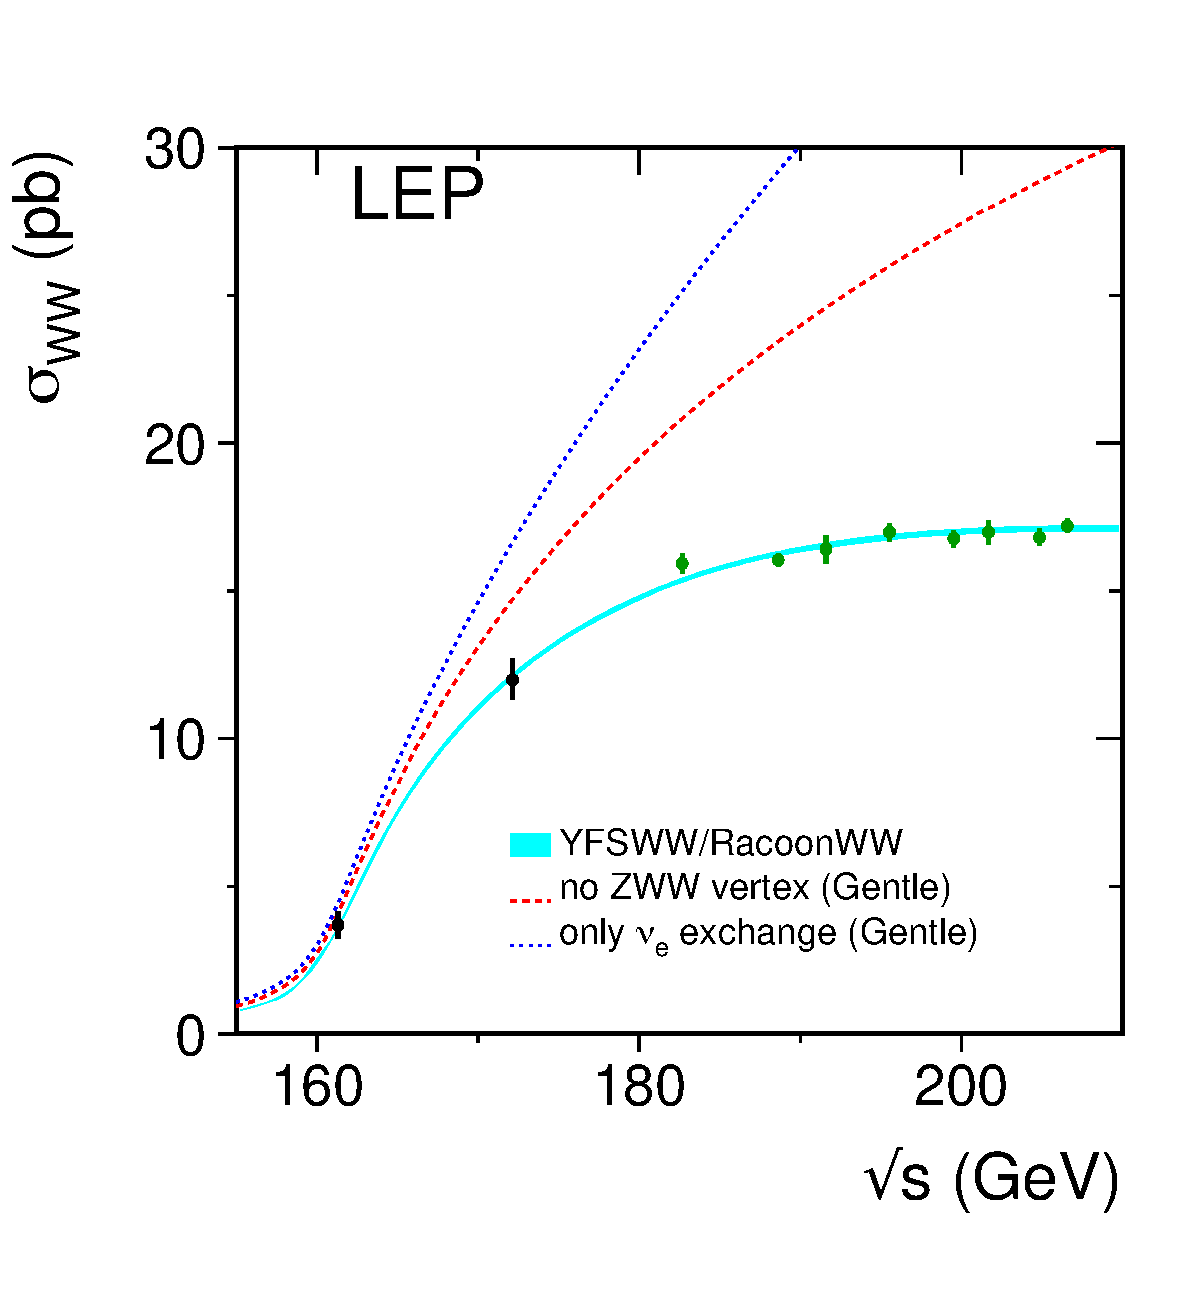
\includegraphics[width=0.6\textwidth]{Fig/4f_wwxsec_nocouplings_2008}
    \caption{Measurements of the $\PW$-pair production cross-section, compared to the different predictions. The shaded area represents the uncertainty on the theoretical predictions~\cite{Schael:2013ita}. \label{fig:eeWWUnitarity}} 
  \end{center}
\end{figure} 

The cancellation that preserves the unitary of $\EE\to\PWp\PWm$ indicates that the coupling of the $\gamma$, charged- and neutral-currents are related. A unification of the electromagnetic and weak interaction was proposed, and a unified electroweak model was completed by Sheldon Glashow, Abdus Salam, and Steven Weinberg, and now it is called GSW model.

One thing that must be incorporated in the unification is the correspondence between the weak neutral-current and the physical $\cPZ$ boson. The neutral-current previously stated does not couple to RH particles/LH antiparticles, which is in contrast to the experimental evidence that the neutral $\cPZ$ boson couples, not equally, to both LH and RH particles. 
At the first step, a $\text{U(1)}_{Y}$ local gauge symmetry is introduced to replace the U(1) gauge group of the electromegnetism with the transformation
\begin{equation}
\psi(x) \ \to\ \psi^{\prime}(x) = \hat{U(x)}\psi(x) = \exp\bigg[ig^{\prime}\frac{Y}{2}\chi^{\prime}(x)\bigg]\psi(x),
\end{equation}
with a new field $B_{\mu}$ and a new weak hypercharge $Y$.
This new symmetry yields the same interaction term as the U(1) symmetry of the QED in Eq.~\ref{eqn:interactionQED}, 
\begin{equation}
\label{eqn:IntactionHyper}
g^{\prime}\frac{Y}{2}\gamma^{\mu}B_{\mu}\psi.
\end{equation}
The physical photon $\gamma$ and $\cPZ$ boson are expressed as,
\begin{equation}
\label{eqn:Afield}
A_{\mu}=+B_{\mu}\cos\theta_{W} + W_{\mu}^{(3)}\sin\theta_{W},
\end{equation}
\begin{equation}
\label{eqn:Zfield}
Z_{\mu}=-B_{\mu}\sin\theta_{W} + W_{\mu}^{(3)}\cos\theta_{W},
\end{equation}
where the $\theta_{W}$ is the weak mixing angle. The physical QED and weak neutral- current are therefore,
\begin{equation}
\label{eqn:jem1}
j_{em}^{\mu}=j_{Y}^{\mu}\cos\theta_{W} + j_{3}^{\mu}\sin\theta_{W},
\end{equation}
\begin{equation}
\label{eqn:jz1}
j_{Z}^{\mu}=-j_{Y}^{\mu}\sin\theta_{W} + j_{3}^{\mu}\cos\theta_{W},
\end{equation}
with the weak neutral-current $j_{3}$ of Eq.~\ref{eqn:WeakCur5} and the current associated with the interaction term $j_{Y}$ of Eq.~\ref{eqn:IntactionHyper} 
\begin{equation}
j_{Y}^{\mu}=\frac{1}{2}g^{\prime}Y_{\Pe_{L}}\bar{\Pe}_{L}\gamma^{\mu}\Pe_{L}
+\frac{1}{2}g^{\prime}Y_{\Pe_{R}}\bar{\Pe}_{R}\gamma^{\mu}\Pe_{R}
+\frac{1}{2}g^{\prime}Y_{\nu_{L}}\bar{\nu}_{L}\gamma^{\mu}\nu_{L}
+\frac{1}{2}g^{\prime}Y_{\nu_{R}}\bar{\nu}_{R}\gamma^{\mu}\nu_{R}
\end{equation}
On the other hand, the electromagnetic current (of the electron doublet) is simply 
\begin{equation}
\label{eqn:jem2}
j_{em}^{\mu}=Q_{e}e\bar{\Pe}_{L}\gamma^{\mu}\Pe_{L}+Q_{e}e\bar{\Pe}_{R}\gamma^{\mu}\Pe_{R}.
\end{equation}
The underlying symmetry group of the electroweak sector, as described in GSW model, is $U(1)_{Y} \times SU(2)_{L}$. In order to preserve the invariance under $U(1)_{Y}$ and $SU(2)_{U}$ local gauge transformation, the hypercharges of particles in a weak isospin doublet should be the same.
Having this argument and equating each component of the Eq.~\ref{eqn:jem1} with $j_{3}^{\mu}$ and $j_{Y}^{\mu}$ substituted and Eq.~\ref{eqn:jem2}, the weak hypercharge can be expressed as a linear combination of the electromagnetic charge $Q$ and the third component of weak isospin $I_{W}^{(3)}$
\begin{equation}
\label{eqn:YQI}
Y=2\big(Q-I_{W}^{(3)}\big),
\end{equation}
Relations between the weak coupling $g_{W}$, the hypercharge coupling $g^{\prime}$ and the electric charge can be derived
\begin{equation}
\label{eqn:relation3}
e=g_{W}\sin\theta_{W}=g^{\prime}\cos\theta_{W}.
\end{equation}
The GSW model successfully bridges the couplings of QED, weak, and the hypercharge with the simple relation.
The measurement of the weak mixing angle, in convention, provides the value of $\sin^{2}\theta_{W}$, which is also the ratio of the weak to electromagnetic coupling constant
\begin{equation}
\label{eqn:relation4}
\sin^{2}\theta_{W}=\frac{\alpha}{\alpha_{W}}=\frac{e^{2}}{g^{2}_{W}}\sim 0.23.
\end{equation}
The coupling of the physical $\cPZ$ boson can be determined similarly. 
From Eq.~\ref{eqn:jz1}, the current of the interaction between the $\cPZ$ boson and a fermion (with flavor $f$) can be written as 
\begin{equation}
\label{eqn:currentZff}
\begin{split}
j_{Z}^{\mu} & = g_{Z}\big(I_{W}^{(3)}-Q_{f}\sin^{2}\theta_{W}\big)\bar{u}_{L}\gamma^{\mu}u_{L}-g_{Z}\big(Q_{f}\sin^{2}\theta_{W}\big)\bar{u}_{R}\gamma^{\mu}u_{R}\\
& \equiv g_{Z}\big(c_{L}\bar{u}_{L}\gamma^{\mu}u_{L}+c_{R}\bar{u}_{R}\gamma^{\mu}u_{R}\big) \\
\end{split}
\end{equation}
where $u_{L(R)}$ is the spinor of LH (RH) states, $c_{L}=I_{W}^{(3)}-Q_{f}\sin^{2}\theta_{W}$ and $c_{R}=-Q_{f}\sin^{2}\theta_{W}$ indicating the strengths of the coupling, and the coupling of the physical $\cPZ$ boson defined as
\begin{equation}
\label{eqn:couplingZ}
g_{Z}=\frac{g_{W}}{\cos\theta_{W}}=\frac{e}{\sin\theta_{W}\cos\theta_{W}}.
\end{equation}
As stated previously, the physical $\cPZ$ boson does couple to LH and RH particles, however, unequally. This is intuitively reasonable, as the current associated with the $\cPZ$ boson is the mixture of the weak and $\text{U(1)}_{Y}$ interactions, where the former one couples only to LH particles but the latter one equally couples to LH and RH particles.

In 1967, Steven Weinberg obtained the formula for the $\PW$ and $\cPZ$ boson masses~\cite{PhysRevLett.19.1264}, with the $\theta_{W}$ which had not yet been determined then. In the following years, the $\theta_{W}$ was measured in various experiments, and in 1982 the masses of the $\PW$ and $\cPZ$ bosons were predicted to be $m_{\PW}=82\pm 2\GeVcc$ and $m_{\cPZ}=92\pm 2 \GeVcc$. In 1983, Carlos Rubbia and his group discovered the $\PW$ and the $\cPZ$ boson~\cite{ARNISON1983103,ARNISON1984241} with measured masses $m_{\PW}=80.403\pm 0.029\GeVcc$ and $m_{\cPZ}=91.188\pm 0.002\GeVcc$. Experiments later on also confirmed the couplings. The GSW model is now considered as one of the most important successes in the SM. 

Despite the triumph of the electroweak unification, it did have some questions regarding the whole mechanism. First of all, Eq.~\ref{eqn:Afield} and \ref{eqn:Zfield} demonstrate that the fields of $U(1)_{Y}$ and $SU(2)_{L}$ are mixed to give physical bosons. The underlying nature of this mixture was unclear. Secondly, four electroweak gauge bosons have different masses, especially when comparing the photon with other three massive particles. This fact seems to contradict the physical picture that both electromagnetic and weak interactions are manifestations of a more fundamental electroweak interaction. The problem with the masses happens also on the fermions. In Eq.~\ref{eqn:LagQED}, the mass term in the QED Lagrangian can be expressed in the chiral states
\begin{equation}
\label{eqn:FermionMass_QEDLag}
\begin{split}
-m\bar{\psi}\psi & = -m\bar{\psi}\bigg[\frac{1}{2}(1-\gamma^{5})+\frac{1}{2}(1+\gamma^{5})\bigg]\psi \\
& = -m\bar{\psi}\bigg[\frac{1}{2}(1-\gamma^{5})\psi_{L}+\frac{1}{2}(1+\gamma^{5})\psi_{R}\bigg] \\
& = -m\big(\bar{\psi}_{R}\psi_{L}+\bar{\psi}_L\psi_{R}\big). 
\end{split}
\end{equation}
In the $\text{SU(2)}_{L}$ gauge transformation of the weak interaction, LH particles transform as doublets while RH particles as singlets. Eq.~\ref{eqn:FermionMass_QEDLag} obviously does not follow the required gauge invariance.
Thirdly, a problem was found: the unitarity violation of the scattering process $\PWp\PWm\to\PWp\PWm$. An overview of the $\PW\PW$ scattering process can be found in Ref.~\cite{Szleper:2014xxa}. The original calculation for the amplitude included the diagrams, shown in Fig.~\ref{fig:WWWWscattering1}. The unitarity violation results from the longitudinal polarized states of $\PW$ boson and the process $\PW_{L}\PW_{L}\to\PW_{L}\PW_{L}$. The issue is solved by introducing a new scalar particle to mediate the $\PW\PW$ process. The diagrams are shown in Fig.~\ref{fig:WWWWscattering_Higgs}.
All the above three problems necessitate a new mechanism, which is now called the Higgs mechanism, with its manifestation, the Higgs boson. 
\begin{figure}[!ht]
  \begin{center}  
    \includegraphics[width=0.67\textwidth]{Fig/WWWWscattering}\\
    \caption{The leading order diagrams for $\PWp\PWm\to\PWp\PWm$ scattering process. \label{fig:WWWWscattering1}}  
  \end{center}
\end{figure}

\begin{figure}[!ht]
  \begin{center}  
    \includegraphics[width=0.67\textwidth]{Fig/WWWWscattering_Higgs}\\
    \caption{The diagrams for $\PWp\PWm\to\PWp\PWm$ scattering process with a scalar boson as mediator. \label{fig:WWWWscattering_Higgs}}  
  \end{center}
\end{figure}

\subsection{The Higgs mechanism}
The Higgs mechanism was proposed back to 1964 by Robert Brout and François Englert, Peter Higgs, and Gerald Guralnik, C. R. Hagen, and Tom Kibble~\cite{PhysRevLett.13.321,PhysRevLett.13.508,PhysRevLett.13.585}.

Before formally introducing the Higgs mechanism in the SM, a single scalar field $\phi$ is used as an example to illustrate the concept. Consider the potential of the form
\begin{equation}
V(\phi) = \frac{1}{2}\mu^{2}\phi^{2} + \frac{1}{4}\lambda\phi^{4}.
\end{equation}
The corresponding Lagrangian is given by 
\begin{equation}
\begin{split}
\mathcal{L}_{ex} & = \frac{1}{2}(\partial_{\mu}\phi)(\partial^{\mu}\phi)- V(\phi) \\
& = \frac{1}{2}(\partial_{\mu}\phi)(\partial^{\mu}\phi) - \frac{1}{2}\mu^{2}\phi^{\mu} - \frac{1}{4}\lambda\phi^{4}.
\end{split}
\end{equation}
In this example Lagrangian, the term of $(\partial_{\mu}\phi)(\partial^{\mu}\phi)$ can be associated with the kinematic energy of the scalar particle. The term of $\phi^{2}$ can be read as the mass of the particle (strictly to say, when $\mu^{2}>0$, it is the coefficient of the $\phi^{2}$ term that associates to the mass). The $\phi^{4}$ term is identified as self-interactions of the scalar field.

The vacuum state is the lowest energy state of the field. In the field theory, the particles state (or the excitations of the field) can be obtained by applying perturbations of the field around the vacuum state. 
In order to have minima for the potential, the $\lambda$ must be positive. When $\mu^{2}>0$, the minimum of the potential happens to be at $\phi=0$. When $\mu^{2}<0$, the term can no longer be interpreted as mass, and the potential now has two degenerate minima at $\phi=\pm v=\pm \mid \sqrt{\frac{-\mu^{2}}{\lambda}} \mid$. 
One needs to arbitrarily select one of the degenerate states as the ground state, then the ground state no longer preserves the symmetry of the Lagrangian. This way to obtain the asymmetric vacuum state is known as \emph{spontaneous symmetry breaking}.

In the SM, the Higgs mechanism is embedded in the $\text{U(1)}_{Y}\times\text{SU(2)}_{L}$ local gauge symmetry of the electroweak sector.
As the Higgs mechanism is required to generate masses of the electroweak gauge bosons, one of the scalar fields must be neutral (therefore termed as $\phi^{0}$), and the other must be charged ($\phi^{+}$ and $\phi^{-}=(\phi^{+})^{\ast}$) to give the longitudinal polarization states of the $\PW$ bosons\footnotemark.
\footnotetext{Before the Higgs mechanism, the gauge bosons do not have masses. Hence, they can only have transverse polarization states. After acquiring the masses, gauge bosons become massive particles, which can have longitudinal polarization state.}
The simplest Higgs model, which has four degrees of freedom and consists of two complex scalar fields, is placed in a weak isospin doublet, 
\begin{equation}
\label{eqn:HiggsModel}
\phi=\begin{pmatrix}
  \phi^{+} \\
  \phi^{0}  
 \end{pmatrix}
 =\frac{1}{\sqrt{2}}\begin{pmatrix}
  \phi_{1}+i\phi_{2} \\
  \phi_{3}+i\phi_{4}  
 \end{pmatrix}
 .
\end{equation}
The Lagrangian of this doublet of fields is 
\begin{equation}
\label{eqn:Lagrangian_Higgs}
\mathcal{L}=(\partial_{\mu}\phi)^{\dagger}(\partial^{\mu}\phi) - V(\phi),
\end{equation}
To preserve the invariance under the $\text{U(1)}_{Y}\times\text{SU(2)}_{L}$ local gauge transformation, the derivative in the Lagrangian should be replaced by the covariant derivative of the form
\begin{equation}
\label{eqn:covderivative_Higgs}
\partial_{\mu}\ \to\ D_{\mu}=\partial_{\mu}+ig_{W}\boldsymbol{T}\cdot\boldsymbol{W}_{\mu}+ig^{\prime}\frac{Y}{2}B_{\mu},
\end{equation}
where $\boldsymbol{T}=\frac{1}{2}\sigma$ are the three generators of the SU(2) group.
The Higgs potential is of the form
\begin{equation}
\label{eqn:Higgspotential}
V(\phi) = \mu^{2}\phi^{\dagger}\phi + \lambda(\phi^{\dagger}\phi)^{2},
\end{equation}
where $\lambda$ is positive.
The visualization of the Higgs field is shown in Fig.~\ref{fig:HiggsPotential}.
\begin{figure}[!ht]
  \begin{center}  
    \includegraphics[width=0.45\textwidth]{Fig/HiggsPotential_MT1}\\
    \caption{The Higgs potential for $\mu^{2}<0$. \label{fig:HiggsPotential}}  
  \end{center}
\end{figure}
The potential is spherically symmetric, and thus the original Lagrangian is spherically symmetric.
For $\mu^{2}<0$, the potential has infinite degenerate minima
\begin{equation}
\label{eqn:Higgspotential}
\phi^{\dagger}\phi = \frac{1}{2}(\phi_{1}^{2}+\phi_{2}^{2}+\phi_{3}^{2}+\phi_{4}^{2})=\frac{v^{2}}{2}=-\frac{\mu^{2}}{2\lambda}.
\end{equation}
For the neutral photon to be massless after the symmetry breaking, the vacuum state is chosen to be
\begin{equation}
\label{eqn:Vacuum_Higgs}
\phi^{\text{vacuum}}=\frac{1}{\sqrt{2}}\begin{pmatrix}
  0 \\
  v  
 \end{pmatrix}
 .
\end{equation}
The symmetry of the original Lagrangian is broken, given that a particular ground state is selected among the degenerate states.
A field $\eta$ is introduced when applying the perturbation around the vacuum state 
\begin{equation}
\label{eqn:phi_Higgs}
\phi^{\text{vacuum}}=\frac{1}{\sqrt{2}}\begin{pmatrix}
  \phi_{1}+i\phi_{2} \\
  v + \eta + i\phi_{4} 
 \end{pmatrix}
 .
\end{equation}
By substituting Eq.~\ref{eqn:phi_Higgs} into the Lagrangian, however, will produce massless Goldstone bosons and terms associated with the couplings between the massive gauge fields and the Goldstone fields. An important fact is that every choice of the gauge transformation, as long as it follows correct form, will not break the symmetry of the Lagrangian. Therefore, a clever way to eliminate the Goldstone fields from the Lagrangian is to choose a gauge transformation called \emph{Unitary gauge}, and after which the complex scalar fields will be entirely real. The Higgs doublet after the Unitary gauge is written as
\begin{equation}
\label{eqn:phi_Higgs_UniGauge}
\phi^{\text{vacuum}}=\frac{1}{\sqrt{2}}\begin{pmatrix}
  0 \\
  v + h 
 \end{pmatrix}
 ,
\end{equation}
where $\eta$ is replaced by $h$, which represents the physical field. After expanding all the terms of the Lagrangian, the masses of gauge bosons can be identified as the coefficients of the quadratic in the gauge fields.

In the Higgs doublet, the lower component is neutral ($Q=0$) and has $I_{W}^{(3)}=-\frac{1}{2}$, therefore the whole doublet has weak hypercharge $Y=1$. 
Expanding the term $(D_{\mu}\phi)^{\dagger}(D^{\mu}\phi)$
\begin{equation}
\label{eqn:DmuDmu}
\begin{split}
(D_{\mu}\phi)^{\dagger}(D^{\mu}\phi) = & \frac{1}{2}(\partial_{\mu}h)(\partial^{\mu}h)+\frac{1}{8}g_{W}^{2}\big(W_{\mu}^{(1)}+iW_{\mu}^{(2)}\big)\big(W^{(1)\mu}-iW^{(2)}\mu\big)(v+h)^{2} \\	
& + \frac{1}{8}\big(g_{W}W_{\mu}^{(3)}-g^{\prime}B_{\mu}\big)\big(g_{W}W^{(3)\mu}-g^{\prime}B^{\mu}\big)(v+h)^{2}
\end{split}
.
\end{equation}
one can identify the quadratic terms as 
\begin{equation}
\label{eqn:quadterm}
\frac{1}{8}v^{2}g_{W}^{2}\bigg(W_{\mu}^{(1)}W^{(1)\mu}+W_{\mu}^{(2)}W^{(2)\mu}\bigg)+\frac{1}{8}v^{2}\bigg(g_{W}W_{\mu}^{(3)}-g^{\prime}B_{\mu}\bigg)\bigg(g_{W}W^{(3)\mu}-g^{\prime}B^{\mu}\bigg)
\end{equation}
Identify the mass of the $\PW$ boson by comparing
\begin{equation}
\frac{1}{2}m_{\PW}^{2}W_{\mu}^{(1)}W^{(1)\mu}=\frac{1}{8}v^{2}g_{W}^{2}W_{\mu}^{(1)}W^{(1)\mu},
\end{equation}
therefore
\begin{equation}
\label{eqn:WbosonMass}
m_{\PW}=\frac{1}{2}g_{W}v.
\end{equation}
The mass the physical $\PW$ boson is determined by the coupling constant of the $SU(2)_{L}$ gauge interaction $g_{W}$ and the vacuum expectation value of the Higgs field $v$.

The second term in Eq.~\ref{eqn:quadterm} is associated with the neutral $W^{(3)}$ and $B$ fields, and can be written as
\begin{equation}
\label{eqn:quadterm_neutral}
\begin{split}
\frac{1}{8}v^{2}\bigg(g_{W}W_{\mu}^{(3)}-g^{\prime}B_{\mu}\bigg)&\bigg(g_{W}W^{(3)\mu}-g^{\prime}B^{\mu}\bigg) = \\
& \frac{1}{8}v^{2}\begin{pmatrix}
  W_{\mu}^{(3)} & B_{\mu}
 \end{pmatrix}
 \begin{pmatrix}
  g_{W}^{2} & -g_{W}g^{\prime} \\
  -g_{W}g^{\prime} & g^{\prime 2}
 \end{pmatrix}
 \begin{pmatrix}
  W^{(3)\mu} \\
  B^{\mu}
 \end{pmatrix}
\end{split}
\end{equation}
The matrix (referred to as mass matrix) appearing in the equation is non-diagonal, showing that the off-diagonal elements couple the $W^{(3)}$ and $B$ fields and allow them to mix.
The physical boson fields (termed as $Z_{\mu}$ and $A_{\mu}$) correspond to the eigenstates of the mass matrix, which can be obtained by solving the characteristic equation 
\begin{equation}
\text{det}(\boldsymbol{M}-\lambda I) = (g_{W}^{2}-\lambda)(g^{\prime 2}-\lambda)-g_{W}^{2}g^{\prime 2} = 0.
\end{equation}
As a result, the eigenvalues $\lambda = 0\ \text{or}\ g_{W}^{2}+g^{\prime 2}$ with the eigenstates
\begin{equation}
\label{eqn:physicalfield_AZ}
\begin{split}
& A_{\mu} = \frac{g^{\prime}W_{\mu}^{(3)}+g_{W}B_{\mu}}{\sqrt{g_{W}^{2}+g^{\prime 2}}} ,\ \ m_{A}=0\ (\text{photon}) \\
& Z_{\mu} = \frac{g_{W}W_{\mu}^{(3)}-g^{\prime}B_{\mu}}{\sqrt{g_{W}^{2}+g^{\prime 2}}} ,\ \ m_{\cPZ}=\frac{1}{2}v\sqrt{g_{W}^{2}+g^{\prime 2}}\ (\cPZ\ \text{boson})
\end{split}
.
\end{equation}
Now, by defining the ratio of the coupling as
\begin{equation}
\label{eqn:tanthetaW}
\frac{g^{\prime}}{g_{W}}=\tan\theta	_{W},
\end{equation}
Eq.~\ref{eqn:physicalfield_AZ} can be expressed as
\begin{equation*}
\begin{split}
& A_{\mu}=+B_{\mu}\cos\theta_{W} + W_{\mu}^{(3)}\sin\theta_{W} \\
& Z_{\mu}=-B_{\mu}\sin\theta_{W} + W_{\mu}^{(3)}\cos\theta_{W}.
\end{split}
\end{equation*}
Eq.~\ref{eqn:Afield} and \ref{eqn:Zfield} are retained.
With Eq.~\ref{eqn:tanthetaW}, the mass of the physical $\cPZ$ boson is
\begin{equation}
m_{\cPZ}=\frac{1}{2}\frac{g_{W}}{\cos\theta_{W}}v.
\end{equation}
Combining with the $\PW$ boson mass from Eq.~\ref{eqn:WbosonMass}, one would obtain
\begin{equation}
\frac{m_{\PW}}{m_{\cPZ}}=\tan\theta_{W}.
\end{equation}
The mass of the Higgs boson $m_{\PH}$ can be identified as the quadratic term in the Higgs boson field which is generated by the potential $V(\phi)$ in the Lagrangian,
\begin{equation}
m_{H}^{2}=2\lambda v^{2}.
\end{equation}

In Eq.~\ref{eqn:DmuDmu}, the gauge boson fields appears in the form of $VV(v+h)^{2}$, where $V$ stands for gauge fields. 
The $VVv^{2}$ terms relate to the mass of the gauge bosons, and the $VVvh$ and $VVhh$ terms represent the triple and quartic couplings between the Higgs bosons and the gauge bosons.
From the weak theory, the physical $\PW$ bosons are constructed as linear combination of the $W^{(1)}$ and $W^{(2)}$, as shown in Eq.~\ref{eqn:Wboson}. Hence, the second term in Eq.~\ref{eqn:DmuDmu} associated with the $W^{(1)}$ and $W^{(2)}$ can be rewritten as 
\begin{equation}
\frac{1}{4}g_{W}^{2}W_{\mu}^{-}W^{+\mu}(v+h)^{2}=\frac{1}{4}g_{W}^{2}v^{2}W_{\mu}^{-}W^{+\mu}+\frac{1}{2}g_{W}^{2}vW_{\mu}^{-}W^{+\mu}h+\frac{1}{4}g_{W}^{2}W_{\mu}^{-}W^{+\mu}hh.
\end{equation}
The first terms gives the masses of $\PW$ boson as stated previous, the second term represents the triple $\PH\PWp\PWm$ coupling, and
the third term gives rise to the quartic $\PH\PH\PWp\PWm$ coupling.
The coupling strength of the $\PH\PWp\PWm$ vertex is 
\begin{equation}
g_{\PH\PW\PW}=\frac{1}{2}g_{W}^{2}v=g_{W}m_{\PW}.
\end{equation}
Similarly, the coupling $\PH\cPZ\cPZ$ can be derived $g_{\PH\cPZ\cPZ}=\frac{g_{W}}{\cos\theta_{W}}m_{\cPZ}\equiv g_{Z}m_{cPZ}$.
\emph{The couplings of the Higgs boson and the gauge bosons are proportional to the mass of the gauge bosons}. 
%Fig.~\ref{fig:HVVcouplings} shows the triple couplings of the Higgs boson to the $\PW$ and $\cPZ$ bosons.
%\begin{figure}[!ht]
%  \begin{center}  
%    \includegraphics[width=0.7\textwidth]{Fig/HVVcouplings}
%    \caption{the triple couplings of the Higgs boson to the $\PW$ and $\cPZ$ bosons. \label{fig:HVVcouplings}}  
%  \end{center}
%\end{figure} 

As mentioned previously, the fermion mass term $-m\bar{\psi}\psi=-m\big(\bar{\psi}_{R}\psi_{L}+\bar{\psi}_{L}\psi_{R}\big)$ is not invariant under $\text{SU(2)}_{L}\times \text{U(1)}_{Y}$ transformation, since the RH and LH fermions transform differently
\begin{equation}
\begin{split}
& \text{LH doublet fermions}\ :\ \psi_{L}\ \to\ \psi_{L}^{\prime}=\psi_{L}\mathrm{e}^{ig_{W}\boldsymbol{T}\cdot\boldsymbol{W}+ig^{\prime}\frac{Y}{2}B} \\
& \text{RH singlet fermions}\ :\ \psi_{R}\ \to\ \psi_{R}^{\prime}=\psi_{R}\mathrm{e}^{ig^{\prime}\frac{Y}{2}B}
\end{split}
.
\end{equation}
The solution is to construct a \emph{singlet} under $\text{SU(2)}_{L}\times \text{U(1)}_{Y}$ in the Lagrangian.
Consider an infinitesimal SU(2) local transformaion on the SU(2) doublet $\phi$ of the Higgs fields,
\begin{equation}
\phi\to\phi^{\prime}=(I+ig_{W}\boldsymbol{\epsilon}(x)\cdot\boldsymbol{T})\phi,
\end{equation} 
where $\boldsymbol{T}$ are generators of the SU(2) group. 
The LH doublets $L$ undergoes the same transformation
\begin{equation}
\begin{split}
& L\to L^{\prime}=(I+ig_{W}\boldsymbol{\epsilon}(x)\cdot\boldsymbol{T})L \\
& \bar{L}=L^{\dagger}\gamma^{0}\to \bar{L}^{\prime} = \bar{L}(I-ig_{W}\boldsymbol{\epsilon}(x)\cdot\boldsymbol{T})
\end{split}
\end{equation}
It is clear that a term of $\bar{L}\phi$ is invariant under the $\text{SU(2)}_{L}$ transformation, or in other word, a singlet under $\text{SU(2)}_{L}\times \text{U(1)}_{Y}$. The effects of the transformation on the $\phi$ and $\bar{L}$ compensate to each other.
Combining the $\bar{L}\phi$ with RH singlet $R$ also results in a singlet under $\text{SU(2)}_{L}\times \text{U(1)}_{Y}$ (The conjugate of the combination is also a singlet).
Conseqently, a term in the Lagrangian of the form $-y_{f}(\bar{L}\phi R+ \bar{R}\phi^{\dagger}L)$ possesses the $\text{SU(2)}_{L}\times \text{U(1)}_{Y}$ gauge symmetry.
The Lagrangian, after spontaneous symmetry breaking and in the unitary gauge, is now 
\begin{equation}
\label{eqn:Lagrangian_fermionmass}
\mathcal{L}_{\text{fermion mass}} = -\frac{y_{f}}{\sqrt{2}}v(\bar{\ell}f_{R}+\bar{f}_{R}\ell)-\frac{y_{f}}{\sqrt{2}}(\bar{\ell}f_{R}+\bar{f}_{R}\ell).
\end{equation}
where $y_{f}$ is a constant known as \emph{Yukawa coupling}.
The first term corresponds to the fermion masses, $m_{\ell}=\frac{y_{f}v}{\sqrt{2}}$, representing the coupling of the fermions to the Higgs field through the non-zero vacuum expectation value. The second term corresponds to the interaction between the fermions and the physical Higgs boson.

The non-zero vacuum expectation value appears only in the lower component of the Higgs doublet, thus only fermions in the lower component of the SU(2) doublet (charged fermions and down-type quarks) can acquire masses, which is obviously not the case.
The way to give masses to up-type quarks is to construct the conjugate doublet of the Higgs field $\phi_{c}$ which transforms in the same way as the doublet $\phi$
\begin{equation}
\phi_{c}=-i\sigma_{2}\phi^{\ast}=\begin{pmatrix}
  -\phi^{0\ast} \\ 
  \phi^{-}
 \end{pmatrix} 
 = 
 \begin{pmatrix}
  -\phi_{3}+i\phi_{4} \\ 
  \phi_{1}-i\phi_{2}
  \end{pmatrix} 
\end{equation}
The Lagrangian of the up-type quark masses is the same as Eq.~\ref{eqn:Lagrangian_fermionmass} except $\phi$ now is replaced by $\phi_{c}$. 
Consequently, the Lagrangian, after the symmetry breaking, is
\begin{equation}
\label{eqn:Lagrangian_uptypemass}
\mathcal{L}_{\text{up-type quark masses}} = -\frac{y_{f,\ \text{up}}}{\sqrt{2}}v(\bar{u}u_{R}+\bar{u}_{R}u)-\frac{y_{f,\ \text{up}}}{\sqrt{2}}(\bar{u}u_{R}+\bar{u}_{R}u).
\end{equation}
where the up-type quark masses can be identified as $m_{\text{up}}=\frac{y_{f,\ \text{up}}v}{\sqrt{2}}$.
The Yukawa coupling of the fermions to the Higgs field is jointly written as
\begin{equation}
y_{f}=\frac{\sqrt{2}m_{f}}{v},
\end{equation}
and its value is determined to be consistent with the observed fermion masses.

The neutrino masses are yet another story. The possible mechanism to account for the neutrino masses was first introduced in Ref.~\cite{GellMann:1980vs,PhysRevLett.44.912}, and is now known as the seesaw mechanism. This mechanism will not be discusses in this thesis. 

A review of the Higgs boson production at the LHC will be introduced in the next sub-section. 

\subsection{The production of the Higgs boson and its decays}
The main production processes at the hadron collider are gluon-gluon fusion (ggF), vector boson fusion (VBF, or qqH), associated vector boson production (VH), and associated top quark pair production (ttH). The diagrams for these production modes are shown in Fig.~\ref{fig:higgsdiags} and the Higgs boson production cross-sections at the center-of-mass frame energy $\sqrt{s}=13\TeV$ are is shown in Fig.~\ref{fig:higgsXS}~\cite{LHCHXSWG}. 
The profound results of the deep inelastic scattering experiments showed that the momentum of the proton is not only carried by its three valence quarks, but also by the gluons that mediate the strong interaction between the quarks. In such a high energy collision at the LHC, the majority of energy is the carried by gluons, and hence the hard processes are dominantly produced by the gluon-gluon interactions.

\begin{figure}[!ht]
  \begin{center}  
    \includegraphics[width=0.3\textwidth]{Fig/Higgs_ggF}~
    \includegraphics[width=0.3\textwidth]{Fig/Higgs_VBF}\\
    \includegraphics[width=0.3\textwidth]{Fig/Higgs_ZWH}~
    \includegraphics[width=0.3\textwidth]{Fig/Higgs_ttH}\\
    \caption{The diagrams for dominant production modes. (Top left) gluon-gluon fusion; (Top right) vector boson fusion; (Bottom left) associated vector boson production; (Bottom right) associated top quark pair production. \label{fig:higgsdiags}}  
  \end{center}
\end{figure} 

\begin{figure}[!ht]
  \begin{center}  
    \includegraphics[width=0.6\textwidth]{Fig/plot_13tev_H_sqrt}\\
    \caption{The SM Higgs boson production cross sections at $\sqrt{s}=13\TeV$ as a function of the Higgs boson mass~\cite{LHCHXSWG}.\label{fig:higgsXS}}  
  \end{center}
\end{figure} 

Since the Higgs boson is the manifestation of the Higgs mechanism which gives fundamental particles masses, in principal it can decay into all particles, if it is kinematically allowed. The decay probability is interpreted as branching ratio. The branching ratio of the most important decay channels as function of the Higgs boson mass are shown in Fig.\ref{fig:higgsBR}. In the following paragraphs, I will discuss the main decay channels of the Higgs boson. 

\begin{figure}[!ht]
  \begin{center}  
    \includegraphics[width=0.6\textwidth]{Fig/Higgs_BR_LM}\\
    \caption{The SM Higgs boson decay branching ratios~\cite{LHCHXSWG}. \label{fig:higgsBR}}  
  \end{center}
\end{figure} 

The Higgs boson cannot decay into top quarks as the top quark is too heavy~\cite{LHCTOPWG}. The coupling between the Higgs boson and the top quark $y_{t}$ is then realized in terms of the ttH production and loops of virtual top quarks in the ggF production or in the decays to the massless particles, such as $\HGG$ and $\PH\to\Pg\Pg$. The combined measurement of the rate of Higgs boson production through gluon-gluon fusion and of the $\HGG$ decay with LHC Run1 data suggested that the Higgs boson coupling to top quarks is consistent with SM prediction within uncertainties~\cite{Khachatryan:2016vau}. A measurement of the production rate of the tree-level ttH process can provide further information as to whether there exists non-SM particles in the loops that introduce terms compensating for other deviations from the SM. The analysis is very difficualt, as the top-quark decays to a $\PW$ bosons and b-quark, and shortly afterwards the $\PW$ decays hadronically to two jets or leptonically to a lepton and a neutrino. Both the ATLAS and CMS Collaboration have recently observed this production channel, and established the confirmation of the tree-level coupling of the Higgs boson to top quarks with the combined analyses of datasets collected at $\sqrt{s}=7$, 8, and 13$\TeV$~\cite{Aaboud:2018urx,Sirunyan:2018hoz}. The best-fit signal strength $\hat{\mu}$ from the ATLAS measurement is $1.32^{+0.28}_{-0.26}(\text{Total})\ \pm 0.18(\text{Stat.})\ ^{+0.21}_{-0.19}(\text{Syst.})$, and from the CMS is $1.26^{+0.31}_{-0.26}(\text{Total})\ \pm 0.16(\text{Stat.})\ ^{+0.27}_{-0.22}(\text{Syst.})$. The ATLAS obtained a significance of 6.3 standard deviations ($\sigma$) relative to the background-only hypothesis, where the expected significance is $5.1\sigma$. The CMS also obtained the observed significance of $5.2\sigma$ with the expected significance is $4.2\sigma$. The Higgs-top coupling can also be probed in the search for the production of Higgs boson in association with a single top quark. The production cross-section of this process is not only sensitive to the absolute values of the modifiers of the Higgs-top coupling, $\kappa_{t}$, and the coupling of vector bosons to the Higgs boson, $\kappa_{V}$, but also to their relative signs with respect to those predicted in the SM. Hence, it provides additional information toward the nature of the Higgs boson. The CMS Collaboration performed this search with data collected in 2016~\cite{CMS-PAS-HIG-18-009}, and the results showed that the observed data favor positive sign of the coupling.

%\begin{figure}[!ht]
%  \begin{center}  
%    \includegraphics[width=0.56\textwidth]{Fig/figaux_02_ttHATLAS}~
%    \includegraphics[width=0.44\textwidth]{Fig/CMS-HIG-17-035_Figure_001_ttHCMS}~
%    \caption{The best-fit signal strength $\hat{\mu}$ from both the ATLAS and CMS results. \label{fig:ttH_Observation}}  
%  \end{center}
%\end{figure} 
The largest branching ratio of the Higgs boson of mass $m_{\PH}=125\GeV$ is to bottom quarks, with $\mathcal{BR}(\PH\to\bbbar)\approx 58.2\%$. The measurement of the rate of the $\PH\to \bbbar$ decay offers a direct test to the magnitude of $\PH\cPqb\cPqb$ coupling, while the relative sign of the coupling can be determined by the decay process $\PH\to\Upsilon +\gamma$, where the $\Upsilon$ is the bound state of the b quarks~\cite{Bodwin:2013gca}. 
%In this channel, there are two hadronic jets in the final states, and hence the inclusive signal is overwhelmed by QCD multijets background $\Pp\Pp\to \bbbar+X$. 
In order to suppress the QCD backgrounds, the analysis is designed to search for the VH production where a W or Z boson decays leptonically, corresponding to five independent channels: $\cPZ(\ell\ell)\PH$, $\PW(\ell\nu)\PH$, and $\cPZ(\nu\nu)\PH$ where $\ell=\re, \mu$. A multivariate regression technique~\cite{Aaltonen:2011bp,Khachatryan:2015ota,Aad:2014xzb} is applied to calibrate the measured energy of the b-tagged jets to improve the dijet mass resolution, after which the mass resolution is approximately 10--15\%. The CMS Collaboration performs the search, and the combination with Run1 measurement results in an observed (expected) significance is 3.8 (3.8)$\sigma$. The corresponding signal strength $\hat{\mu}=1.06^{+0.31}_{-0.29}$~\cite{Sirunyan:2017elk}. The ATLAS Collaboration announces the first observation of this channel with data corresponding to an integrated luminosity of $79.8\fbinv$ collected in Run2 at $\sqrt{s}=13\TeV$~\cite{ATLAS-CONF-2018-036}. A combination with other production modes of the Higgs boson is performed for $\PH\to \bbbar$ decay mode, which yields an observed (expected) significance of 5.4 (5.5) $\sigma$. The signal strength $\hat{\mu}=1.01^{+0.20}_{-0.20}$.

The $\PH\to\TT$ decay mode has been considered as the only accessible leptonic decay mode that probes the coupling of the Higgs boson to the fermionic sector. It can also be used to constrain CP violation in the VBF production~\cite{Aad:2016nal} and provide sensitivity to CP violation in the Higgs boson coupling to leptons~\cite{Berge:2015nua}. This decay benefits from a favorable signal-to-background conditions than the $\PH\to \bbbar$ decay, however, slightly worse mass resolution of $\approx 10 - 20\%$, resulting from the inaccuracy of the momentum reconstruction of the $\PGt$ lepton. The $\PGt$ lepton can decay leptonically as $\PGt\to\nu_{\tau}\ell\bar{\nu}_{l}$ where $\ell=\re, \mu$, and hadronically to charged or neutral pions. The analyses from both the ATLAS and CMS utilizes the four most sensitive $\PGt\PGt$ final states: $\re\mu$, $\re\PGt_{h}$, $\mu\PGt_{h}$, and $\PGt_{h}\PGt_{h}$, where $\PGt_{h}$ denotes the hadronic decay. The ATLAS Collaboration reports the signal strength $\hat{\mu}=1.09^{+0.36}_{-0.30}$ with an observed (expected) significance of 6.4 (5.4) $\sigma$ with a combined analysis with $\sqrt{s}=$7, 8, and 13\TeV data~\cite{ATLAS-CONF-2018-021}. The CMS Collaboration also obtains the signal strength $\hat{\mu}=1.09^{+0.27}_{-0.26}$ with an observed (expected) significance of 5.9 (5.9) $\sigma$ in combination with Run1 data~\cite{Sirunyan:2017khh}.

Prior to the discovery of the Higgs boson, the decay mode $\PH\to\PW\PW$ was considered the most sensitive channel in the mass range around the $\PW\PW$ threshold of 160\GeV, and thus was important to the exclusion in such range. The $\PH\to\PW\PW^{*}\to\ell\nu\ell\nu$ analysis profits from the fact that it has large branching fraction and has a relatively low-background final state. As a result, this decay channel has very good sensitivity to most production processes, in particular ggF and VBF. However, the presence of neutrinos in the final state prevents the full reconstruction of the Higgs boson mass, and hence worse mass resolution of $\approx 20\%$. The different-flavor leptonic decay mode $\re\mu$ has the largest branching fraction, is the least affected by background processes, and therefore is the most sensitive channel of the analysis. The ATLAS Collaboration provides results of ggF and VBF production with 2016 data separately~\cite{ATLAS-CONF-2018-004}. For the ggF production the signal strength $\hat{\mu}=1.21^{+0.22}_{-0.21}$ with an observed (expected) significance of 6.3 (5.2) $\sigma$, while for the VBF the signal strength $\hat{\mu}=0.62^{+0.37}_{-0.36}$ with an observed (expected) significance of 1.9 (2.7) $\sigma$. The CMS Collaboration reports the signal strength $\hat{\mu}=1.28^{+0.18}_{-0.17}$ with an observed (expected) significance of 9.1 (7.1) $\sigma$, combining all considered channels~\cite{Sirunyan:2018egh}.

The $\PH\to\cPZ\cPZ^{*}\to 4\ell\ (\ell=\re\ \text{or}\ \mu)$ decay has low branching fraction, but fortunately has the lowest background contamination, resulting in very good sensitivity. It provides the direct probe in constraining the $\PH\cPZ\cPZ$ coupling. The precise reconstruction of the final state products allows the complete determination of the kinematics of the reconstructed Higgs boson with mass resolution of $\approx 1 - 2\%$, which makes it one of the most important channels to measure the properties of the Higgs boson. The ATLAS and CMS Collaborations have both performed analyses for this channel with the Run1 data to determine the mass and spin-parity of the boson~\cite{Chatrchyan:2013mxa,Chatrchyan:2012jja,Khachatryan:2014kca,Aad:2014eva,Aad:2015mxa}, its width~\cite{Khachatryan:2014iha,Khachatryan:2015mma,Aad:2015xua}, the fiducial cross sections [22, 23], and the tensor structure of its interaction with a pair of neutral gauge bosons~\cite{Khachatryan:2014kca,Aad:2015mxa,Khachatryan:2015mma}. These measurements provided results that are so far consistent with the SM predictions. The CMS Collaboration provides results, based on the combined data collected in 2016 and 2017, of the signal strength $\hat{\mu}=1.06^{+0.15}_{-0.13}$~\cite{CMS-PAS-HIG-18-001}. The ATLAS Collaboration reports the signal strength $\hat{\mu}=1.18^{+0.13}_{-0.13}$~\cite{ATLAS-CONF-2018-018}. A model-independent measurement of the Higgs boson width is performed by the CMS Collaboration with 2016 data using the $m_{4\ell}$ distribution in the range $105 < m_{4\ell} < 140\GeV$, and is able to constrain the width to be $\Gamma_{\PH}<1.10\ (1.60)\GeV$ at 95\% confidence level (CL) for observed (expected) value~\cite{Sirunyan:2017exp}.

Despite the small branching fraction predicted by the SM, the $\HGG$ decay provides a clean final state, two energetic photons, with an invariant mass peak that can be reconstructed with high precision with mass resolution of $\approx 1 - 2\%$. Consequently, this channel was one of the most important channels for the Higgs boson discovery and first measurements of its properties~\cite{Khachatryan:2014ira,Aad:2014eha}. Since the $\HGG$ decay proceeds mainly through $\PW$- and top-loop processes, interference effects make its branching fraction sensitive to the relative sign of the fermion and vector boson couplings. The differential cross sections enables us to test the perturbative QCD predictions for Higgs boson production, and can be used to probe the spin and CP properties of the Higgs boson. The CMS Collaboration provides the results using 2016 data of the signal strength $\hat{\mu}=1.18^{+0.17}_{-0.14}$~\cite{Sirunyan:2018ouh}, while the ATLAS Collaboration obtains $\hat{\mu}=0.99^{+0.14}_{-0.14}$. The interpretation of the coupling measurements from both collaborations shows that the observed data favors the positive sign of the coupling~\cite{Sirunyan:2018kta,Aaboud:2018xdt}. The ATLAS Collaboration also tries to investigate the strength and tensor structure of the Higgs boson interactions using an effective Lagrangian, which introduces additional CP-even and CP-odd interactions~\cite{Aaboud:2018xdt}, but no significant new physics contributions are observed.

The decay of $\PH\to\cPZ/\gamma^{*}+\gamma$ shares almost the same diagrams as that of the $\HGG$ decay, where in the former one a $\cPZ$ boson or a virtual photon $\gamma^{*}$ is radiated from the loop. Measurement of this rare decay can enhance the current understanding of the nature of the Higgs boson, and can also provide an alternative way to test if there is any beyond standard model (BSM) couplings induced in the loop diagrams. A brief summary of these extension of SM can be found in Ref.~\cite{Sirunyan:2018tbk,Aaboud:2017uhw}. If there exists BSM that is manifested through CP violation, one can also observe the anomaly though a measurement of the forward-backward asymmetry. The ATLAS Collaboration sets an observed (expected) exclusion upper limit on the production cross section times the branching ratio of the $\PH\to\cPZ\gamma$ decay of 6.6 (5.2) times the SM prediction at 95\% CL for a Higgs boson mass $m_{\PH}=125.09\GeV$, while the upper limits from the CMS Collaboration varies between 6.1 and 11.4 (3.9 and 9.1) times the SM value in the mass range of $120<m_{\PH}<130\GeV$~\cite{Sirunyan:2018tbk,Aaboud:2017uhw}. The CMS Collaboration also provides so far the most stringent limit on the $\PH\to\gamma^{*}\gamma$ decay, varying between 1.4 and 4.0 (2.1 and 2.3) times the SM prediction in the range of $120<m_{\PH}<130\GeV$~\cite{Sirunyan:2018tbk}.

The rare decay $\PH\to\mu\mu$ offers the best possibility to measure the Higgs coupling to second-generation fermions at the LHC. The expected branching fraction for a Higgs boson mass $m_{\PH}=125.09\GeV$ is $\mathcal{BR}(\PH\to\mu\mu)\approx 2.2\ten{-4}$~\cite{deFlorian:2016spz} which is roughly one order of magnitude smaller than the $\PH\to\cPZ/\gamma^{*}+\gamma$ decay, owing to the small Yukawa coupling of the muon to the Higgs field. The CMS Collaboration sets the observed (expected) upper limit on the signal strength of 2.92 (2.16) times the SM prediction, with combination of 7, 8, and 13\TeV data~\cite{Sirunyan:2018hbu}, while the ATLAS Collaboration reports an upper limit of 2.1 (2.0) times the SM values~\cite{ATLAS-CONF-2018-026}.

The other decay of the Higgs boson to second-generation fermions that was searched for is the $\PH\to\ccbar$ process. It is commonly considered impossible to discover this channel even in high luminosity run of the LHC (HL-LHC) due to the small branching fraction, large background in hadron collider, and jet flavor identification inefficiency~\cite{Perez:2015aoa,Perez:2015lra}. Nevertheless, direct search for the $\PH\to\ccbar$ decay is important in the long-term perspective, as the development of the charm-tagging technique and the direct constraint of the Higgs-charm coupling would be valuable inputs to the next generation of particle colliders. The ATLAS Collaboration presents the first search for this process with data collected in 2016, utilizing the $\cPZ\PH$ production with the subsequent decay of the Z boson to dilepton. The observed (expected) upper limit on the production cross-section $\sigma(\Pp\Pp\to\cPZ\PH)\times\mathcal{BR}(\PH\to\ccbar)$ is found to be $2.7\ (3.9^{+2.1}_{-1.1})\pb$ at the 95\% CL, corresponding to an observed (expected) upper limit on  the signal strength $\hat{\mu}<110\ (150^{+80}_{-40})$~\cite{Aaboud:2018fhh}.

\subsection{The measurement of the Higgs coupling}
The ATLAS and CMS Collaborations both reported the observation of a new boson with a mass of $m_{\PH}=125.09\pm 0.21(\text{stst.})\pm 0.11(\text{syst.})\GeV$~\cite{Aad:2015zhl} in 2012, and subsquent mesurements revealed its Higgs-boson-like properties~\cite{Chatrchyan:2012jja,Khachatryan:2014kca,Aad:2012tfa,Chatrchyan:2012xdj,Chatrchyan:2013lba,Aad:2015gba,Khachatryan:2014jba,Aad:2013xqa}. One of the important analyses, and most related to this thesis, is the measurement of the Higgs coupling.  A combined measurement were performed by ATLAS and CMS with data collected at 7 and 8\TeV~\cite{Khachatryan:2016vau}, and the CMS Collaboration provides the latest results with 13\TeV data~\cite{CMS-PAS-HIG-17-031}. The results from CMS with 13\TeV data will be shown in the following paragraphs.

The inputs of the analysis are the four main production processes introduced previously, decay channels to bosons $\PH\to\cPZ\cPZ,\ \PW\PW,\ \PGg\PGg$, and to fermions $\PH\to\PGt\PGt,\ \bbbar,\ \PGm\PGm$. In this work, a so-called $\kappa-$framework~\cite{Heinemeyer:2013tqa} is used\footnotemark. 
\footnotetext{It was referred to as Interim framework in the cited reference.}
Within the framework, there are assumptions made such that the production and decay of the Higgs boson can be factorized and parametrized as 
\begin{equation}
\sigma_{i}\cdot\mathcal{BR}^{f}=\frac{\sigma_{i}(\overrightarrow{\kappa})\cdot\Gamma^{f}(\overrightarrow{\kappa})}{\Gamma_{\PH}},
\end{equation}
where $\Gamma_{\PH}$ is the total width of the Higgs boson and $\Gamma^{f}$ is the partial width for Higgs boson decay to the final state $f$. Coupling modifiers, $\overrightarrow{\kappa}$, are introduced in order to test deviations in the couplings of the Higgs boson to other particles, and are defined as 
\begin{equation}
\kappa_{j}^{2}=\frac{\sigma_{j}}{\sigma_{j}^{\text{SM}}}\ \text{or}\ \kappa_{j}^{2}=\frac{\Gamma^{j}}{\Gamma^{j}_{\text{SM}}},
\end{equation}
where all $\kappa_{j}=1$ in the SM and $j$ denotes the tested production or decay mode.
Tree-level Higgs boson couplings, such as the $\PH-\cPZ,\ \PH-\PW,\ \PH-t,\ \PH-b,\ \PH-\PGt,\ \text{and}\ \PH-\PGm$, are introduced as individual coupling modifiers. For those processes that occur at leading-order (LO) involving box or triangular loop diagrams, the loops are resolved in terms of the corresponding coupling modifiers, weighted by their individual contribution. Interference effects between the different diagrams provide sensitivity to the relative signs of the Higgs boson couplings to different particles. The coupling modifiers $\kappa_{\cPqc}$ and $\kappa_{\PQs}$ are allowed to vary as function of other modifiers, provided that current LHC data are insensitive to these couplings. The constraint on $\kappa_{\cPqc}$ will be introduced separately later. Other coupling modifiers $\kappa_{\PQu}$, $\kappa_{\PQd}$, and $\kappa_{\re}$ are not included in combination given that their magnitudes are marginal. 

There are two parametrization schemes. One is defined such that two additional effective coupling modifiers, $\kappa_{\cPg}$ and $\kappa_{\PGg}$, which describe the loop processes for ggF production and $\HGG$ decay, are introduced to account for the situation that BSM particles may be present in these loops. The other one is to resolve the ggF and $\HGG$ processes as function of remaining coupling modifiers. 
Fig.~\ref{fig:kappaCMS2016_1} shows the summary plots for the $\kappa$-framework model with the resolved loop scheme and the assumption $\mathcal{BR}_{\text{BSM}}=0$. The points indicate the best fit values while the thick and thin horizontal bars show the $1\sigma$ and $2\sigma$ CL intervals, respectively. Without loss of generality, the value of $\kappa_{\PQt}$ is restricted to be positive. For this model, both positive and negative values of $\kappa_{\PW}$, $\kappa_{\cPZ}$, and $\kappa_{\PQb}$ are considered. The result shows that negative values of $\kappa_{\PW}$ are disfavored by more than $2\sigma$. The interference between diagrams of the $\cPZ\PH$ production leads to the break of the degeneracy between signs, and indicates that a positive value of $\kappa_{\cPZ}$ is favored. A negative value of $\kappa_{\PQb}$ is preferred in this model, however, the difference between the best-fit point and the minimum in the positive region is small. 
Fig.~\ref{fig:kappaCMS2016_2} shows the summary plots with effective couplings scheme. In the left figure the constraint $\mathcal{BR}_{\text{BSM}}=\mathcal{BR}_{\text{inv}}+\mathcal{BR}_{\text{undet}}=0$ is imposed, and both positive and negative values of $\kappa_{\PW}$ and $\kappa_{\cPZ}$ are considered. In the right figure a constraint $|\kappa_{V}| \leq 1$, where $\kappa_{V}$ denotes $\kappa_{\cPZ}$ or $\kappa_{\PW}$, is imposed (same sign of $\kappa_{\cPZ}$ and $\kappa_{\PW}$), while $\mathcal{BR}_{\text{inv}} > 0$ and $\mathcal{BR}_{\text{undet}} > 0$ are free parameters. The preferred sign of the $\kappa_{\PW}$, opposite to the first scheme, is negative. In Fig.~\ref{fig:kappaCMS2016_3}, left plot shows the scan of the test statistic as a function of $\mathcal{BR}_{\text{inv}}$, and the right plot shows the 68\% and 95\% CL contours for $\mathcal{BR}_{\text{inv}}$ vs. $\mathcal{BR}_{\text{undet}}$, indicating the 95\% CL upper limits of $\mathcal{BR}_{\text{inv}}<0.22$ and $\mathcal{BR}_{\text{undet}}<0.36$.

\begin{figure}[!ht]
\begin{center}
\includegraphics[width=0.5\textwidth]{Fig/HIG17031/plot_K1_mm_merged}\\
\caption{Summary for the $\kappa$-framework model with the resolved loop scheme~\cite{CMS-PAS-HIG-17-031}. \label{fig:kappaCMS2016_1}}
\end{center}
\end{figure}

\begin{figure}[!ht]
\begin{center}
\includegraphics[width=0.56\textwidth]{Fig/HIG17031/plot_K2_merged}~
\includegraphics[width=0.44\textwidth]{Fig/HIG17031/plot_K2Undet_merged}\\
\caption{Summary for the $\kappa$-framework model with the effective couplings scheme~\cite{CMS-PAS-HIG-17-031}. \label{fig:kappaCMS2016_2}}
\end{center}
\end{figure}

\begin{figure}[!ht]
\begin{center}
\includegraphics[width=0.535\textwidth]{Fig/HIG17031/scan_pub_observed_K2Undet_BRinv}~
\includegraphics[width=0.465\textwidth]{Fig/HIG17031/plot_BRinvVsBRbsm_N4}\\
\caption{Scan of the test statistic as a function of $\mathcal{BR}_{\text{inv}}$ (left), and 68\% and 95\% CL regions for $\mathcal{BR}_{\text{inv}}$ vs. $\mathcal{BR}_{\text{undet}}$ (right)~\cite{CMS-PAS-HIG-17-031}. \label{fig:kappaCMS2016_3}}
\end{center}
\end{figure}

Another fit is performed using a phenomenological parameterization relating the masses of the fermions and vector bosons to the corresponding modifiers with two parameters, $M$ and $\epsilon$~\cite{Ellis:2012hz,Ellis:2013lra}. In this parametrization, the coupling modifiers, $M$ and $\epsilon$ are related as $\kappa_{F} = \frac{v\cdot m_{f}^{\epsilon}}{M^{1+\epsilon}}$ for fermions and $\kappa_{V} = \frac{v\cdot m_{V}^{2\epsilon}}{M^{1+2\epsilon}}$ for vector bosons, where $v = 246.22\GeV$ is the vacuum expectation value~\cite{Patrignani:2241948}. The SM expectation of $\kappa=1$, corresponds to $(M, \epsilon) = (v, 0)$. 
The left plot in Fig.~\ref{fig:kappaCMS2016_4} shows the $1\sigma$ and $2\sigma$ CL regions in the $(M,\epsilon)$ fit, and the results of the fit using the six modifiers are plotted versus the particle masses on the right-hand side, as well as the result of the $(M,\epsilon)$ fit. A ''reduced`` vector boson coupling $\frac{\sqrt{\kappa_{V}\cdot m_{V}}}{v}$ is shown to represent the couplings of the vector bosons in the same plot. As one can see, the couplings of these six particles to the Higgs boson are consistent within uncertainties with the SM predictions.

\begin{figure}[!ht]
\begin{center}
\includegraphics[width=0.5\textwidth]{Fig/HIG17031/plot_Meps_2D}~
\includegraphics[width=0.5\textwidth]{Fig/HIG17031/plot_Meps_ratio}\\
\caption{(Left) Likelihood scan in the $M-\epsilon$ plane. The best fit point and the $1\sigma$ and $2\sigma$ CL regions are shown, along with the SM prediction. (Right) Result of the phenomenological $(M, \epsilon)$ fit with the loop-resolved scheme of $\kappa$-framework model~\cite{CMS-PAS-HIG-17-031}. \label{fig:kappaCMS2016_4}}
\end{center}
\end{figure}

\subsection*{The Higgs-charm coupling}
As stated previously, a sensitive measurement of Higgs-charm coupling is not feasible in the environment of the LHC. There are still ways to constrain the size of the coupling. Since c- and b-jets share rough similarities, jets originating from charm quarks may be mistagged as b- jets. Hence, with the tagging efficiency of c- and b-jets, one can recast the existing analyses of $\PH\to\bbbar$ to constrain the $\PH\to\ccbar$ rate~\cite{Perez:2015aoa}. This results in a model-independent bound on the charm signal strength of $\mu_{\cPqc}=95^{+90}_{-95}$ with the results of the $\PH\to\bbbar$ search in VH production from both ATLAS and CMS Collaborations. 
Both ATLAS and CMS Collaboration give a model-independent bound on the Higgs total width from the invariant-mass distribution of the $\PH\to\cPZ\cPZ^{*}$ and $\HGG$in the Run1 analyses. This bound on the total width can be used to constrain the Higgs-charm coupling by assuming the entire Higgs width is formed by $\PH\ccbar$. With this method, the upper bounds at 95\% CL with the CMS results is $\kappa_{\cPqc}<120$ and with the ATLAS results is $\kappa_{\cPqc}<150$. 
A method that relies on the measurements of transverse momentum distributions of Higgs boson was proposed to determine the limit on the coupling modifier $\kappa_{\cPqc}$~\cite{Bishara:2016jga}. Fig.~\ref{fig:HiggsPt_KappaC} shows the impact of the coupling modifier $\kappa_{\cPqc}$ on the normalized $p_{\text{T}}^{\PH}$ spectrum in inclusive Higgs production. This letter takes the \pt spectrum from the ATLAS combined measurement of $\HGG$ and $\PH\to\cPZ\cPZ^{*}$ decays with Run1 $\sqrt{s}=8\TeV$ data, and obtains the bounds on $\kappa_{\cPqc}$ at 95\% CL of $\kappa_{\cPqc}\in [-16,18]$. The spectrum of the $p_{\text{t}}^{\PH}$ at $\sqrt{s}=13\TeV$ is expected to be slightly harder than that of $\sqrt{s}=8\TeV$, thus will enhance the sensitivity to $\kappa_{\cPqc}$ at ongoing LHC runs as well as possible future hadron colliders at higher energies. The CMS Collaboration applies this method with the distributions from $\HGG$ and $\PH\to\cPZ\cPZ^{*}$ analyses using data collected in 2016 to set limit on the constrain of $\kappa_{\cPqc}$~\cite{CMS-PAS-HIG-17-028}. Fig.~\ref{fig:HiggsPt_KappaC_CMS2016} shows the simultaneous fit results for $\kappa_{\PQb}$ and $\kappa_{\cPqc}$. On the left plot, 1 and $2\sigma$ deviation contours for the combined ($\HGG$ and $\PH\to\cPZ\cPZ^{*}$) fit to data and for $\HGG$ and $\PH\to\cPZ\cPZ^{*}$ separately, assuming coupling dependency of the branching fractions, while the right plot assumes freely floating branching fractions in the fit. The observed (expected) constraints on $\kappa_{\cPqc}$ are
\begin{equation}
-4.3 < \kappa_{\cPqc} < 4.3\ (-5.4 < \kappa_{\cPqc} < 5.3)\ \text{(coupling dependent }\mathcal{BR}),
\end{equation}
\begin{equation}
-18.0 < \kappa_{\cPqc} < 22.9\ (-15.7 < \kappa_{\cPqc} < 19.3)\ \text{(freely floating }\mathcal{BR}).
\end{equation}
If the branching fractions are fixed to the SM expectations, the expected constraint will be
\begin{equation}
-8.7< \kappa_{\cPqc} < 10.6\ \text{(SM branching fractions)}.
\end{equation}

Rare exclusive decays of the Higgs boson to mesons in association with a photon can be used to explore these couplings. For example, the $\PH\to\JPsi\ \gamma$ decay can probe the Higgs boson coupling to the charm quark~\cite{Bodwin:2013gca}. This decay is the focus in the thesis, and will be discuss in the next section. Using Run1 results of the upper limit on $\PH\to\JPsi\ \gamma$, the bound at 95\% CL is set at $\kappa_{\cPqc}<220$.

\begin{figure}[!ht]
\begin{center}
\includegraphics[width=0.5\textwidth]{Fig/HiggsPt_kappac}~
\caption{The normalized $p_{\text{T}}^{\PH}$ spectrum of inclusive Higgs production at $\sqrt{s}=8\TeV$ with different values of $\kappa_{\cPqc}$~\cite{Bodwin:2013gca}. \label{fig:HiggsPt_KappaC}}
\end{center}
\end{figure}

\begin{figure}[!ht]
\begin{center}
\includegraphics[width=0.5\textwidth]{Fig/CMS-PAS-HIG-17-028_Figure_006-a}~
\includegraphics[width=0.5\textwidth]{Fig/CMS-PAS-HIG-17-028_Figure_006-b}\\
\caption{Simultaneous fit results for $\kappa_{\PQb}$ and $\kappa_{\cPqc}$~\cite{CMS-PAS-HIG-17-028}. \label{fig:HiggsPt_KappaC_CMS2016}}
\end{center}
\end{figure}

In some extensions to the SM, modified $\PH \ccbar$ couplings can arise~\cite{Delaunay:2013pja}. 
For example, within the context of the effective field theory~\cite{Buchmuller:1985jz,Weinberg:1980wa,Contino:2013kra} the $\PH\ccbar$ coupling is modified in the presence of dimension-six operator, leading to only an enhancement of the coupling with respect to the SM at the cutoff scale $\Lambda$, of order tens of $\TeV$, and leaving no other signature of new physics at the LHC.
In the two Higgs doublet model with minimal flavor violation~\cite{Trott:2010iz,Jung:2010ik}, the $\PH \ccbar$ coupling can be significantly enhanced by breaking the flavor symmetry, while other couplings are not severely affected. The composite pseudo-Nambu-Goldstone boson model~\cite{Giudice:2007fh} parametrizes the coupling by the degree of compositeness and compositeness scale, which can be experimentally constrained by the direct search for the charm partner~\cite{Delaunay:2013pwa}.
%In some extension theories beyond the SM, modified $\PH \ccbar$ coupling can arise~\cite{Delaunay:2013pja}. For instance, the effective field theory suggests that an enhancement of the coupling with respect to the SM can appear at cutoff scale $\Lambda$ around tens of \TeV, so that no direct signatures at the LHC can be observed other than a significantly enhanced $\PH \ccbar$ coupling. In the two Higgs doublet model with minimal flavor violation~\cite{Trott:2010iz,Jung:2010ik}, the $\PH \ccbar$ coupling can be significantly enhanced by breaking the flavor symmetry, while other couplings not severely affected. The composite pseudo-Nambu-Goldstone boson model~\cite{Giudice:2007fh} parametrizes the coupling by the degree of compositeness and compositeness scale, which can be experimentally constrained by the direct search of the charm partner~\cite{Delaunay:2013pwa}.

\section{The rare decays $\cPZ/\PH\to\JPsi\ \gamma$}
\subsection{Overview}
%A new boson with a mass of approximately 125\GeV was discovered by the ATLAS and CMS Collaborations at the CERN LHC in 2012~\cite{Chatrchyan2013,Aad:2013xqa,201230,Chatrchyan:2013lba,CMS:2014ega,AtlasProperties,CMS:2015kwa}. 
%Up to now, all measurements of its properties are consistent with those of the Higgs boson of the SM. 
%The Higgs boson Yukawa couplings to the first-- and second--generation quarks are currently weakly constrained.
%Rare exclusive decays of the Higgs boson to mesons in association with a photon can be used to explore these couplings. For example, the $\PH\to\JPsi\ \gamma$ decay can probe the Higgs boson coupling to the charm quark~\cite{Bodwin:2013gca}.
The rare decay of $\PH\to\JPsi\ \gamma$ is one of the proposed ways to probe the Higgs-charm coupling. The corresponding decay of the $\cPZ$ boson, $\cPZ\to\JPsi\ \gamma$, can be used as an experimental benchmark for the $\PH\to\JPsi\ \gamma$ search, given that the mass of the $\cPZ$ boson is not far from that of the Higgs boson, and to test various QCD factorization approaches that are being used in the estimation of branching fractions for hadronic radiative decays of bosons~\cite{GUBERINA1980317,PhysRevD.92.014007,Grossmann:2015lea}.

Both the Higgs and $\cPZ$ boson decays have contributions from direct and indirect processes. In the direct mechanism, $\cPZ$ and Higgs bosons couple to charm quarks, and charm quarks then hadronize to form $\JPsi$ mesons. 
In the indirect mechanism, the Higgs and $\cPZ$ bosons decay through the quark and W boson loops to 
$\gamma\gamma^{*}$, and the $\gamma^{*}$ then converts to a $\ccbar$ resonant state.  
The Feynman diagrams for these decay modes are shown in Fig.~\ref{fig:ZJpsiG_diag}. 
The widths of the decays are expected to be
\begin{equation}
\label{eqn:widthHJpsiG}
\begin{split}
\Gamma_{\PH\to\JPsi\ \gamma} & =\frac{1}{8\pi}\frac{m_{\PH}-m_{\JPsi}}{m_{\PH}} |\mathcal{A}_{\text{direct}}+\mathcal{A}_{\text{indirect}}|^{2} \\
& = \bigg[(11.71\pm 0.17) - \big[(0.659^{+0.085}_{-0.085})+i(0.073^{+0.035}_{-0.035})\big]\kappa_{\cPqc}\bigg]\ten{-10}\GeV \\
& =1.221^{+0.042}_{-0.041}\ten{-8}\GeV,
\end{split}
\end{equation}
\begin{equation}
\label{eqn:widthZJpsiG}
\Gamma_{\cPZ\to\JPsi\ \gamma}=\frac{m_{\cPZ}^{3}}{96\pi m_{\JPsi}^{2}} |\mathcal{A}_{\text{direct}}+\mathcal{A}_{\text{indirect}}|^{2}= 2.236^{+0.377}_{-0.344}\ten{-7}\GeV,
\end{equation}
where in Eq.~\ref{eqn:widthHJpsiG} the equality and numerical results are taken from Ref.~\cite{Bodwin:2013gca,Bodwin:2017wdu}, and those in Eq.~\ref{eqn:widthZJpsiG} are from Ref.~\cite{Bodwin:2017pzj}.
In these theoretical calculations, a framework of the nonrelativistic QCD (NRQCD) factorization~\cite{PhysRevD.51.1125} is used, where the nonperturbative effects are parametrized in terms of the quarkonium light-cone distribution amplitudes (LCDAs)~\cite{PhysRevD.22.2157,Chernyak:1983ej}. These computations will not be discussed in detail here. 
With the total widths of both the Higgs $\Gamma_{\PH}=4.20\MeV$ and $\cPZ$ boson $\Gamma_{\cPZ}=2.4952\GeV$ and $\kappa_{\cPqc}=1$ in the SM, the branching fractions of both decays are then:
\begin{equation}
\mathcal{B}_{\text{SM}}(\PH\to\JPsi\ \gamma)=(3.0^{+0.2}_{-0.2})\ten{-6}.
\end{equation}
\begin{equation}
\mathcal{B}_{\text{SM}}(\cPZ\to\JPsi\ \gamma)=(9.0^{+1.5}_{-1.4})\ten{-8},
\end{equation}
The direct and indirect amplitudes interfere destructively in both decays. In the Higgs decay, the contribution from the indirect process is larger. Only direct process included in the calculation leads to a brancing fractions of $5.28\ten{-8}$, while only indirect diagrams included results in a brancing fractions of $3.25\ten{-6}$. The branching fraction of the $\cPZ$ decay, compared to the Higgs decay, is smaller by 1-2 orders of magnitude. This results from the suppression of the indirect amplitude, which is less than 1\% of the magnitude of direct amplitude, in the $\cPZ$ decay. One qualitative explanation uses the Landau-Yang theorem~\cite{PhysRev.77.242}, which states that the $\cPZ$ boson does not decay to two on-shell photon. This requires that the indirect amplitude tends to zero in the limit $m_{\JPsi}\to 0$.

With the branching fractions shown above, one can obtain
\begin{equation}  
\begin{split}
\sigma(\Pp\Pp\to\PH) \times \mathcal{B}_{\text{SM}}&(\PH\to\JPsi\ \gamma\to\mu\mu\gamma) = \\
& 55\ \text{pb} \times 3.0\times10^{-6} \times 0.059 = 9.8\ten{-3}\ \text{fb},
\end{split}
\end{equation}  
\begin{equation} 
\begin{split}
\sigma(\Pp\Pp\to\cPZ) \times \mathcal{B}_{\text{SM}}&(\cPZ\to\JPsi\ \gamma\to\mu\mu\gamma) =\\
& 5.7\times 10^{4}\ \text{pb} \times 9.0\times10^{-8} \times 0.059 = 3.0\ten{-1}\ \text{fb}.
\end{split}
\end{equation}
where the cross-section of the Higgs boson are summed over the ggF, VBF, VH, and ttH productions, and taken from Ref.~\cite{deFlorian:2016spz}. The cross-section of the $\cPZ$ boson are calculated using $\FEWZ$ 3.1.b2 program~\cite{Li:2012wna}.

\begin{figure}[!ht]\begin{center}
\includegraphics[width=0.4\textwidth]{Fig/ZJpsiG_direct_v2}\\
\includegraphics[width=0.33\textwidth]{Fig/ZJpsiG_Indirect1_v2}~
\includegraphics[width=0.33\textwidth]{Fig/ZJpsiG_Indirect2_v2}~
\includegraphics[width=0.33\textwidth]{Fig/ZJpsiG_Indirect3_v2}\\
\caption{Feynman diagrams for $\cPZ(\PH)\to\JPsi\ \gamma$ decay. The top diagram shows the direct process and the remaining diagrams show the indirect processes.}
\label{fig:ZJpsiG_diag}\end{center}\end{figure}

Deviations from the SM predictions for the couplings can affect the interference terms and may result in changes in the branching fractions. 
For example, the shift in the branching fraction for $\PH\to\JPsi\ \gamma$ can be more than 100\% if the $\PH \ccbar$ coupling deviates from its SM value by more than a factor of 2, as shown in Fig.~\ref{fig:BRShift}. 
Measurements of the direct decay of $\PH\to\ccbar$ leave the overall signs of the couplings undetermined. This ambiguity can be resolved by the interference terms in $\PH\to\JPsi\ \gamma$, providing us with additional information about the Higgs properties.
%Since this Higgs boson decay is sensitive to the $\PH\ccbar$ coupling, a measurement of the branching fraction can verify if the Higgs boson couples to second-generation quarks with the strength predicted by the SM.

\begin{figure}[!ht]
  \begin{center}  
    \includegraphics[width=0.65\textwidth]{Fig/BRShift}\\
    \caption{The relative deviations in the branching fraction for $\PH\to\JPsi\ \gamma$ as function of $\kappa_{\cPqc}$~\cite{Bodwin:2013gca}.  \label{fig:BRShift}}  
  \end{center}
\end{figure}

%\begin{figure}[!ht]
%  \begin{center}  
%    \includegraphics[width=0.35\textwidth]{Fig/HDalitz_1}~
%    \includegraphics[width=0.35\textwidth]{Fig/HDalitz_2}\\
%    \includegraphics[width=0.35\textwidth]{Fig/HDalitz_3}\\
%    \caption{Main diagrams for the Higgs Dalitz decay, $\PH\to\gamma^{*}\gamma\to\mu\mu\gamma$}  
%    \label{fig:FeynmanDiagrams_Dalitz}
%  \end{center}
%\end{figure} 
%
%
%\begin{figure}[!ht]
%  \begin{center}  
%    \includegraphics[width=0.35\textwidth]{Fig/Zmmg1}~
%    \includegraphics[width=0.35\textwidth]{Fig/Zmmg2}
%    \caption{Main diagrams for the Drell-Yan process, $\Pp\Pp\to\cPZ\to\mu\mu\gamma$, which is the background that will exhibit a peak in $\text{m}_{\mu\mu\gamma}$ at the Z boson mass, $m_{\cPZ}$.}  
%    \label{fig:FeynmanDiagrams_Zmmg}
%  \end{center}
%\end{figure}

\subsection{Features of the decays}
Due to the relatively heavy $\cPZ$ and Higgs boson, the $\JPsi$ and $\gamma$ from their decays will have high transverse momenta $\pt$ and energy $\et$ (boosted). The high-$\et$ photon will be produced back-to-back to the $\JPsi$ particle, and hence can be distinguished from backgrounds easily and be identified as an isolated photon. 
Since the $\JPsi$ meson from $\cPZ$ (Higgs) boson decay is boosted, the $\pt$ of the two muons from its decay are anti-correlated. Further, these two muons are very close to each other spatially. Therefore, dedicated strategies for trigger algorithms and both offline reconstruction are needed. 
The photon should be well separated from each muon. This event signature can be utilized to design kinematic requirements such as the angular separation $\Delta R$\footnotemark to reject backgrounds. 
\footnotetext{The coordinate system will be introduced in the next chapter.}

%The background compositions are not complicated. The main irreducible background is the Drell-Yan process, where the photon can either be initial-state radiation (ISR) or final-state radiation (FSR). The reducible backgrounds come from Drell-Yan with jet and inclusive quarkonium production, where the jet in both processes is misidentified as a photon at reconstruction level. 
%$\JPsi$ mesons can come from heavy-flavor hadron decays (These $\JPsi$ mesons will be referred to as non-prompt $\JPsi$). 
%Those $\JPsi$ mesons have longer proper decay time $t$ and decay length $\text{L}_{\text{xy}}$ than those of the $\JPsi$ meson from signal events (The $\JPsi$ from the signal events are therefore called prompt $\JPsi$). 
%These features can be used to examine if the reconstructed $\JPsi$ meson candidate in selected events are promptly produced.  

Fig.~\ref{fig:GenLevel_HJpsiG} shows the distributions of key variables at the generator level. All the distributions shown in the figure are normalized to unity. One can see that, the momenta of muons cover a wide range: the transverse momentum \pt of trailing muon\footnotemark can be less than 10\GeV, while that of leading muon can be greater than 40 and 60\GeV in the $\cPZ$ and Higgs boson decay respectively. The photon can have high transverse energy. The muons and the photon distribute mostly in the central region. The high-$\et$ photon is back-to-back to the dimuon system, while the two muons are close to each other spatially. 
\footnotetext{In the analysis, two muons will be selected in the final state. The one with higher \pt is referred to as leading muon, and the other one is then referred to as trailing or subleading muon.}

\begin{figure}[p]\begin{center}  
\includegraphics[width=0.33\textwidth]{Fig/GenLevel_HJpsiG/plot_ZHJpsiG/ZHJpsiG_mu1Pt}~
\includegraphics[width=0.33\textwidth]{Fig/GenLevel_HJpsiG/plot_ZHJpsiG/ZHJpsiG_mu2Pt}~
\includegraphics[width=0.33\textwidth]{Fig/GenLevel_HJpsiG/plot_ZHJpsiG/ZHJpsiG_phoEt}\\
\includegraphics[width=0.33\textwidth]{Fig/GenLevel_HJpsiG/plot_ZHJpsiG/ZHJpsiG_mu1Eta}~
\includegraphics[width=0.33\textwidth]{Fig/GenLevel_HJpsiG/plot_ZHJpsiG/ZHJpsiG_phoEta}~
\includegraphics[width=0.33\textwidth]{Fig/GenLevel_HJpsiG/plot_ZHJpsiG/ZHJpsiG_dimuPt}\\
\includegraphics[width=0.33\textwidth]{Fig/GenLevel_HJpsiG/plot_ZHJpsiG/ZHJpsiG_dRdimuon}~
\includegraphics[width=0.33\textwidth]{Fig/GenLevel_HJpsiG/plot_ZHJpsiG/ZHJpsiG_dRmu1pho}~
\includegraphics[width=0.33\textwidth]{Fig/GenLevel_HJpsiG/plot_ZHJpsiG/ZHJpsiG_mmgPt}\\
\includegraphics[width=0.33\textwidth]{Fig/GenLevel_HJpsiG/plot_ZHJpsiG/ZHJpsiG_mmgEta}~
\includegraphics[width=0.33\textwidth]{Fig/GenLevel_HJpsiG/plot_ZHJpsiG/ZHJpsiG_mmgRapidity}\\
\caption{The distributions of key variables at generator level in both the Z and Higgs boson decays: 
	$\pt$ and $\et$ of the leading, trailing muon and the photon,
	pseudorapidity $\eta$ of the leading muon and the photon, $\pt$ of the $\JPsi$ meson , angular separation $\Delta \text{R}$ between muons, $\Delta \text{R}$ between the leading muon and the photon, $\pt$ of the $\cPZ$ and Higgs boson, $\eta$ of the $\cPZ$ and Higgs boson, and the rapidity Y of the $\cPZ$ and Higgs boson}  
\label{fig:GenLevel_HJpsiG}\end{center}\end{figure}  

%\begin{figure}[h]\begin{center}  
%\includegraphics[width=0.95\textwidth]{Fig/GenLevel_ZJpsiG/GenLevelStudy_ZJpsigamma_74XvsSummer16}
%\caption{The kinematic distribution of key variables at generator level in $Z\rightarrow J/\psi + \gamma$ decay: 
%	Transverse momenta of the leading/trailing $\pt$ muon and the photon,
%	pseudorapidity of the muons and the photon, distances $\Delta R_{E_{T}a\phi}$ between the two muons and between the muons and the photon. In this figur%e, two signal samples are compared: one produced by Pythia6 and the other by Pythia8.}  
%\label{fig:GenLevel_ZJpsiG}\end{center}\end{figure}  

%\begin{figure}[!ht]\begin{center}
%\includegraphics[width=0.7\textwidth]{Fig/GenLevel_HJpsiG/CosTheta_v4}
%\caption{The distribution of $\text{cos}\Theta$, where $\Theta$ is the angle between the direction of the Higgs and the $\gamma$ in the center-of-mass frame of the Higgs. This angle is derived at generator level.}
%\label{fig:CosTheta_H_gamma}\end{center}\end{figure}

\subsection{Previous results from the ATLAS and CMS Collaborations}
The $\cPZ \to\JPsi\ \gamma$ decay was searched for by the ATLAS Collaboration using the data set collected at $\sqrt{s}=8\TeV$~\cite{Aad:2015sda}. An observed (expected) upper limit on the branching fraction of $2.6\ (2.0^{+1.0}_{-0.6})\ten{-6}$ was reported. 
Searches for the $\PH\to\JPsi\ \gamma$ decay have been performed by the ATLAS and CMS Collaborations using the data set collected at $\sqrt{s}=8\TeV$ respectively~\cite{Aad:2015sda,Run1Paper_Dalitz}. Observed (expected) limits on the branching fraction were $1.5\ (1.2^{+0.6}_{-0.3})\ten{-3}$ from the ATLAS Collaboration and $1.5\ (1.6^{+0.8}_{-0.8})\ten{-3}$ from the CMS Collaborations. Fig.~\ref{fig:ATLAS8TeV} shows the three-body invariant mass $m_{\mu\mu\gamma}$ and $\pt^{\mu\mu\gamma}$ distributions, along with the signal-plus-background fit to observed data collected at $\sqrt{s}=8\TeV$ from ATLAS results. Fig.~\ref{fig:CMS8TeV} shows the non-resonant background fit to the $m_{\mu\mu\gamma}$ distributions observed in data collected at $\sqrt{s}=8\TeV$ with CMS search.
Recently, ATLAS provides results with data collected in 2016 for both decays. An observed (expected) upper limit on the branching fraction of $\cPZ \to\JPsi\ \gamma$ decay is set at $2.3\ (1.1^{+0.5}_{-0.3})\ten{-6}$, and of the $\PH\to\JPsi\ \gamma$ is at $3.5\ (3.0^{+1.4}_{-0.8})\ten{-4}$~\cite{Aaboud:2018txb}.
Fig.~\ref{fig:ATLAS2016} shows the recent results from ATLAS Collaboration.
%The ATLAS Collaboration has also searched for the $\PH\to\ccbar$ decay in the $\Pp\Pp \to \cPZ\PH$ production mode using data collected at $\sqrt{s}=13\TeV$~\cite{Aaboud:2018fhh}, and reported observed (expected) limits on $\sigma/\sigma_{\text{SM}}$ ratio of 110 ($150^{+80}_{-40}$), where the $\sigma_{\text{SM}}$ is the expected SM value for the cross section.

\begin{figure}[!ht]
  \begin{center}  
    \includegraphics[width=0.99\textwidth]{Fig/PreviousResult/fig_01.pdf}\\
    \caption{Previous result of $\cPZ\ (\PH)\to\JPsi\ \gamma$ decay search from the ATLAS Collaboration. The three-body invariant mass $m_{\mu\mu\gamma}$ and $\pt^{\mu\mu\gamma}$ distributions, along with the results of signal-plus-background fit to observed data collected at $\sqrt{s}=8\TeV$~\cite{Aad:2015sda}.  \label{fig:ATLAS8TeV}}  
  \end{center}
\end{figure}

\begin{figure}[!ht]
  \begin{center}  
    \includegraphics[width=0.7\textwidth]{Fig/PreviousResult/CMS-HIG-14-003_Figure_005.pdf}\\
    \caption{Previous result of $\PH\to\JPsi\ \gamma$ decay search from the CMS Collaboration. Non-resonant background fit to the $m_{\mu\mu\gamma}$ distributions observed in data collected at $\sqrt{s}=8\TeV$~\cite{Aad:2015sda}.}  
    \label{fig:CMS8TeV}
  \end{center}
\end{figure}

\begin{figure}[!ht]
  \begin{center}  
    \includegraphics[width=0.99\textwidth]{Fig/fig_04a_ATLAS2016}\\
    \caption{Result of $\cPZ\ (\PH)\to\JPsi\ \gamma$ decay search from the ATLAS Collaboration with data collected at $\sqrt{s}=13\TeV$ in 2016~\cite{Aaboud:2018txb}.\label{fig:ATLAS2016}}  
  \end{center}
\end{figure}
%\begin{figure}[!ht]
%  \begin{center}  
%    \includegraphics[width=0.45\textwidth]{Fig/PreviousResult/fig_02a}~
%    \includegraphics[width=0.45\textwidth]{Fig/PreviousResult/fig_02b}\\
%    \caption{Result of $\PH\to\ccbar$ search in the $\Pp\Pp\to\cPZ\PH$ production mode using data collected at $\sqrt{s}=13\TeV$ from the ATLAS Collaboration.}  
%    \label{fig:ATLASHcc}
%  \end{center}
%\end{figure}